%% jnuthesis 文档类的可选参数有:
%%   nobackinfo 取消封二页导师签名信息.注意,按照南大的规定,是需要签名页的.
%%   phd/master/bachelor 选择博士/硕士/学士论文

% 使用 blindtext 宏包自动生成章节文字
% 这仅仅是用于生成样例文档,正式论文中一般用不到该宏包
\documentclass[bachelor,adobefonts]{jnuthesis}

% 本科课程设计课程名称
\usepackage{graphicx}
\usepackage{subcaption}
\usepackage{algorithm}
\usepackage{algorithmic} 
\renewcommand{\algorithmicrequire}{\textbf{Input:}} 
\renewcommand{\algorithmicensure}{\textbf{Output:}}


\graphicspath{ {images/} }
%%%%%%%%%%%%%%%%%%%%%%%%%%%%%%%%%%%%%%%%%%%%%%%%%%%%%%%%%%%%%%%%%%%%%%%%%%%%%%%
% 设置论文的中文封面

% 如果论文标题过长,可以分两行,第一行用\titlea{}定义,第二行用\titleb{}定义,将上面的\title{}注释掉
\titlea{复杂网络技术在数据挖掘中的应}
\titleb{用}



% 论文作者姓名
\author{汪建海}
% 论文作者学生证号
\studentnum{1030414623}
% 导师姓名职称
\supervisor{方伟}
\supervisorpos{讲师}
% 第二行导师姓名职称,仿照第一行填写,没有则留空
\supervisorb{}
\supervisorbpos{}
% 论文作者的学科与专业方向
\major{计算机科学与技术}
% 论文作者所在院系的中文名称,学士学位论文此处不带“学院”二字
\department{物联网工程}
% 论文作者所在学校或机构的名称.此属性可选,默认值为``江南大学''.
\institute{江南大学}
% 学士学位获得日期,需设置年、月,默认为编译日期.
\bachelordegreeyear{2018}
\bachelordegreemonth{6}
%%%%%%%%%%%%%%%%%%%%%%%%%%%%%%%%%%%%%%%%%%%%%%%%%%%%%%%%%%%%%%%%%%%%%%%%%%%%%%%

%-------------------------------------------------------------------------------
%	CODE INCLUSION CONFIGURATION
%-------------------------------------------------------------------------------
\usepackage{listings}
\newfontfamily\menlo{Menlo}
\usepackage{color}
\lstset{
    columns=fixed,
    breaklines=true,
    numbers=left,                                        % 在左侧显示行号
    frame=single,                                        % 显示背景边框
    % backgroundcolor=\color[RGB]{245,245,244},            % 设定背景颜色
    % keywordstyle=\color[RGB]{40,40,255},                 % 设定关键字颜色
    numberstyle=\footnotesize\color{darkgray},           % 设定行号格式
    % commentstyle=\color[RGB]{0,96,96},                   % 设置代码注释的格式
    % stringstyle=\color[RGB]{128,0,0},                    % 设置字符串格式
    showstringspaces=false,                              % 不显示字符串中的空格
    basicstyle=\small\menlo,
    numberstyle=\scriptsize\menlo,
    xleftmargin=0cm,
    xrightmargin=0cm
}

\begin{document}

%%%%%%%%%%%%%%%%%%%%%%%%%%%%%%%%%%%%%%%%%%%%%%%%%%%%%%%%%%%%%%%%%%%%%%%%%%%%%%%

% 制作中文封面
\maketitle

%%%%%%%%%%%%%%%%%%%%%%%%%%%%%%%%%%%%%%%%%%%%%%%%%%%%%%%%%%%%%%%%%%%%%%%%%%%%%%%
% % 开始前言部分
% \frontmatter

%%%%%%%%%%%%%%%%%%%%%%%%%%%%%%%%%%%%%%%%%%%%%%%%%%%%%%%%%%%%%%%%%%%%%%%%%%%%%%%
% 论文的中文摘要
\begin{abstract}
自然语言理解是自然语言处理乃至人工智能领域亟待研究重点与难点,
对其研究在理论上和实际应用上都有重要的意义.
随着深度学习的发展,基于循环神经网络(RNN)、长短期记忆网络(LSTM)等的序列建模方式已经成为了
自然语言处理的主流方法.
但是这些深度学习模型需要大规模训练数据,并且将复杂的语言分析和理解
过程简化成“黑盒子”,难以融合先验语言知识,进而使模型缺乏可解释性.

本文尝试将先验文本语言学知识引入传统深度学习模型中,提出了融合句法结构的深度神经网络.
该模型通过依存句法分析工具获得文本的句法子结构,
然后将文本的语义表示和结构表示分别通过两个独立的LSTM模型,
再将子结构输出的加权平均结果与主文本句子的输出结果相融合,
从而实现利用句法结构信息对句子表示增强,最后将这个增强表示送入后续的神经网络中以完成文本分类、机器翻译等文本理解应用.

通过在文本理解的基础性任务文本分类上进行对照实验,
得出融合模型相对传统深度学习模型具有以下两个主要优点:
(1)由于引入了语言学知识,在小规模数据集上有明显优势;在大规模数据集上也有一定优势,模型有较好的鲁棒性.
(2)通过Attention机制可视化文本中不同结构的重要程度,使得模型具有一定的可解释性.

在实验中还对融合模型的Attention机制和融合方式开展了进一步的研究.最终在AGNews数据集上,
融合模型相对于LSTM模型在测试集上的正确率提升了2.5\%.

% 中文关键词.关键词之间用中文全角分号隔开,末尾无标点符号.
\keywords{文本理解;依存句法结构;深度学习 ;融合模型}
\end{abstract}

%%%%%%%%%%%%%%%%%%%%%%%%%%%%%%%%%%%%%%%%%%%%%%%%%%%%%%%%%%%%%%%%%%%%%%%%%%%%%%%
% 论文的英文摘要



\begin{englishabstract}
Natural language understanding is an urgent task in the field of natural language processing and artificial intelligence.
The research is of great significance in both theory and practice.
In recent years, with the development of deep learning, the sequential modeling methods based on Recurrent Neural Network (RNN) and Long Short Term Memory Network (LSTM) have been established.
The mainstream method of natural language processing.
But these deep learning models require massive training of data and complex language analysis and understanding.
The process is simplified into “black box”, which is difficult to combine with the prior language knowledge, thus making the model lack of interpretability.
  
This paper attempts to introduce the knowledge of prior text linguistics into the traditional deep learning model, and puts forward the deep neural network of syntactic structure.
This model acquires the syntactic substructure of text by means of the dependency syntactic analysis tool.
Then the semantic representation and structure of the text are represented by two separate LSTM models.
The weighted average result of the substructure output is combined with the output result of the main text sentence.
In this way, the sentence is enhanced by using syntactic structure information. Finally, this enhancement is sent to the subsequent neural network to complete the application of text classification, machine translation and other text understanding.
  
By conducting a controlled experiment on the basic task text categorization of text comprehension,
It is concluded that the fusion model has two main advantages:
(1) due to the introduction of linguistic knowledge, there are obvious advantages in the small-scale data set; There are some advantages in large-scale data sets, and the model has good robustness.
(2) the importance of different structures in the visual text of the Attention mechanism makes the model have certain interpretability.
  
In the experiment, the Attention mechanism and fusion mode of the fusion model were further studied. Finally, in the AGNews data set,
The accuracy of the fusion model in the test set was increased by 2.5\% compared with the LSTM model.
% 英文关键词.关键词之间用英文半角逗号隔开,末尾无符号.
\englishkeywords{Text understanding;Structure of dependency syntax; Deep learning; Fusion model}
\end{englishabstract}

%%%%%%%%%%%%%%%%%%%%%%%%%%%%%%%%%%%%%%%%%%%%%%%%%%%%%%%%%%%%%%%%%%%%%%%%%%%%%%%
% 生成论文目次
\tableofcontents

%%%%%%%%%%%%%%%%%%%%%%%%%%%%%%%%%%%%%%%%%%%%%%%%%%%%%%%%%%%%%%%%%%%%%%%%%%%%%%%
% 开始正文部分
\mainmatter

%%%%%%%%%%%%%%%%%%%%%%%%%%%%%%%%%%%%%%%%%%%%%%%%%%%%%%%%%%%%%%%%%%%%%%%%%%%%%%%
% 学位论文的正文应以《绪论》作为第一章

%第一章绪论
\chapter{绪论}\label{chapter_introduction}
\section{研究背景和意义}
自然语言处理(Natural Language Processing,NLP)是研究计算机处理人类语言的一门技术,也是人工智能(Artificial Intelligence,AI)最初发展的切入点和当前关注的焦点.

人工智能整体上自下而上可以分为3个层次,分别是运算智能、感知智能、认知智能.
最后也是最高级的认知智能主要就表现在自然语言处理水平上.
如果语言处理理解能够取得突破,认知智能领域中的知识推理也能够获得发展,
这样就能推动整个人工智能的发展,从而使得更多的应用场景能够落地.
所以自然语言处理也一直被看成人工智能这个皇冠上的明珠.

而自然语言理解(Natural Language Understanding,NLU)技术则是对语义信息的深层次挖掘和处理,是NLP技术当前研究的重点和难点.
广义的自然语言理解可以分为两类,第一类是针对口语内容的理解,如语音识别,语音解析和语音合成;
第二类是对书面文本的理解,也是本文主要讨论的内容,即本文题中的文本理解(Text understanding).
人工智能,自然语言处理,自然语言理解和文本理解的关系可以表示为下图.

\begin{figure}[h!]
  \centering
    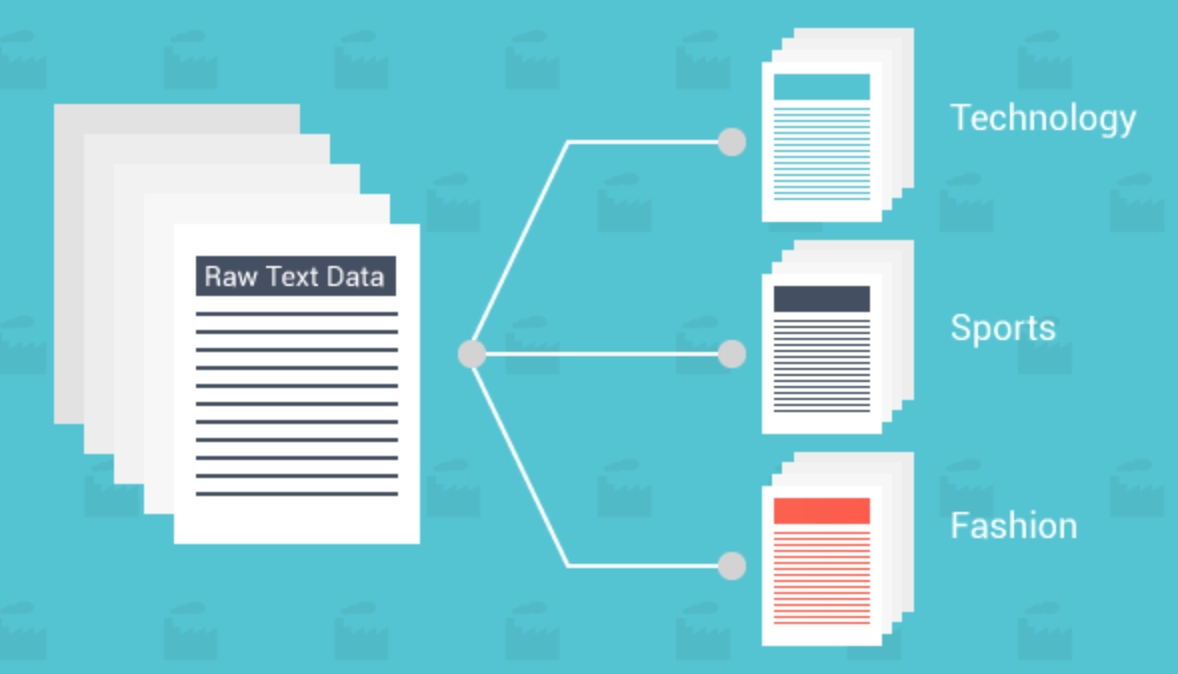
\includegraphics[width=\linewidth]{wenbenfenlei.png}
  \caption{人工智能,自然语言处理,自然语言理解和文本理解的关系}
\end{figure}

文本理解技术是众多高级NLP应用c不合或缺的一项核心技术,
这些应用包括文本自动分类、结构化信息抽取、长文本自动摘要、
机器翻译、问答系统等.

(1)文本分类:文本分类是文本理解最为基础性的应用也是最为广泛应用的应用.
例如:对垃圾邮件进行过滤,自动对新闻进行主题分类和文本情感色彩识别等.
这个应用核心步骤主要包括:文本的特征提取和类别最优匹配.

(2)信息抽取:信息抽取 是把文本里包含的信息进行结构化处理,变成表格一样的组织形式.
输入信息抽取系统的是原始文本,输出的是固定格式的信息点.
信息点从各种各样的文档中被抽取出来,然后以统一的形式集成在一起.

(3)自动摘要:随着互联网的高速发展,随着而来的文本信息量也在几何倍的曾在,人们每天
疲于面对微博、短信、文摘、微信等海量的文本信息.
而自动文本摘要就提供了一个高效的解决方案,
可以从原文本中提炼出简洁而重要的信息.

(4)机器翻译:机器翻译是程序化得将源语言和目标语言之间进行自动转换的过程,
这是自然语言发展的起点也是最终的目标.这项应用,不仅具有很高的学术研究价值,
同时面对全球化的发展,机器翻译将会极大的促进不同语言的人进行经济、文化和政治等多方面的交流.

(5)问答系统:问答系统本质上是最为高级的搜索方式,它能用准确、简洁的自然语言回答用户用自然语言提出的问题.
这种交互一直认为是最自然的人机交互方式,随着苹果Siri,微软Cortana,天猫智能客服的推出,智能问答系统成为备受关注的热点研究方向.

(6)舆情分析:舆情是指社会空间中群众对社会事件的产生、发展、结果的评价、态度、感情的综合体现.
舆情的来源现阶段主要是互联网,包括贴吧、论坛、微博等平台.
舆情分析涉及到网络文本内容挖掘,观点意见挖掘,所以是个综合性的复杂技术.

\begin{figure}[h!]
  \centering
  \begin{subfigure}[b]{0.4\linewidth}
    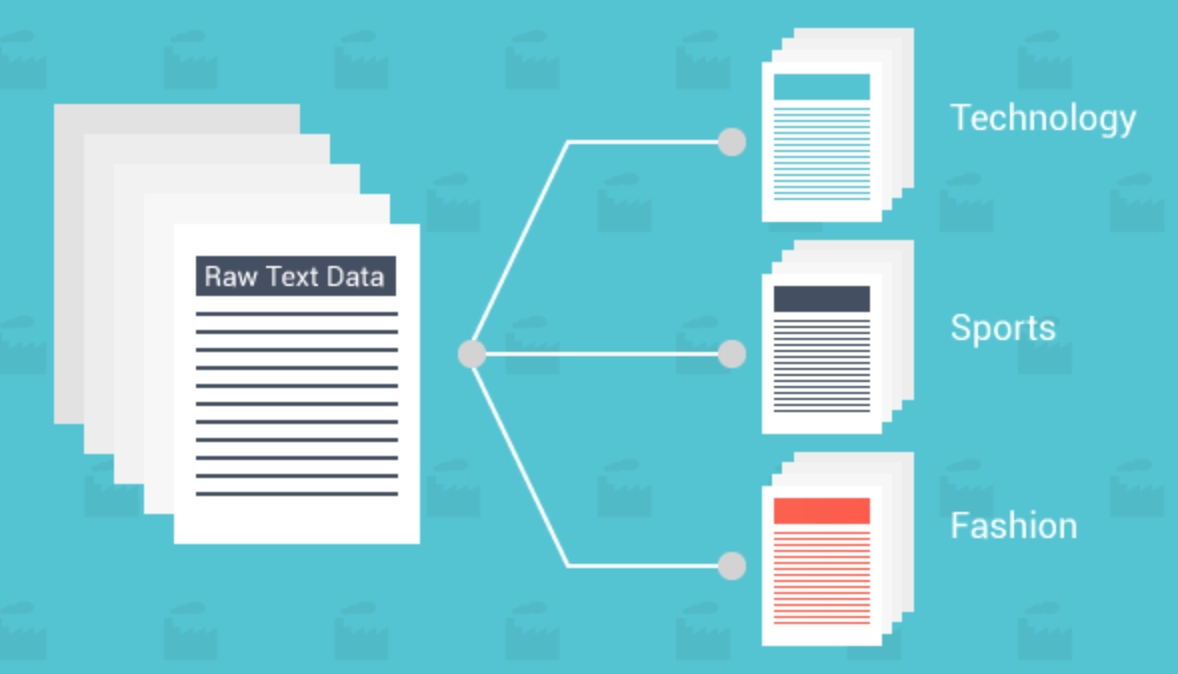
\includegraphics[width=\linewidth]{wenbenfenlei.png}
    \caption{文本分类}
  \end{subfigure}
  \begin{subfigure}[b]{0.4\linewidth}
    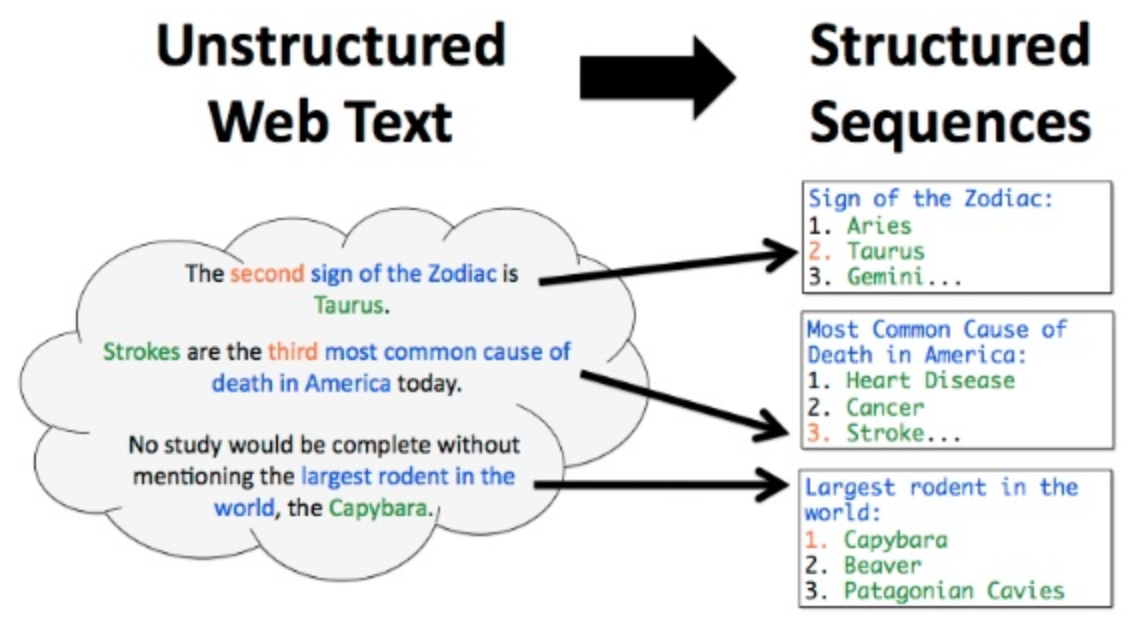
\includegraphics[width=\linewidth]{xinxichouqu.png}
    \caption{信息抽取}
  \end{subfigure}
  \begin{subfigure}[b]{0.4\linewidth}
    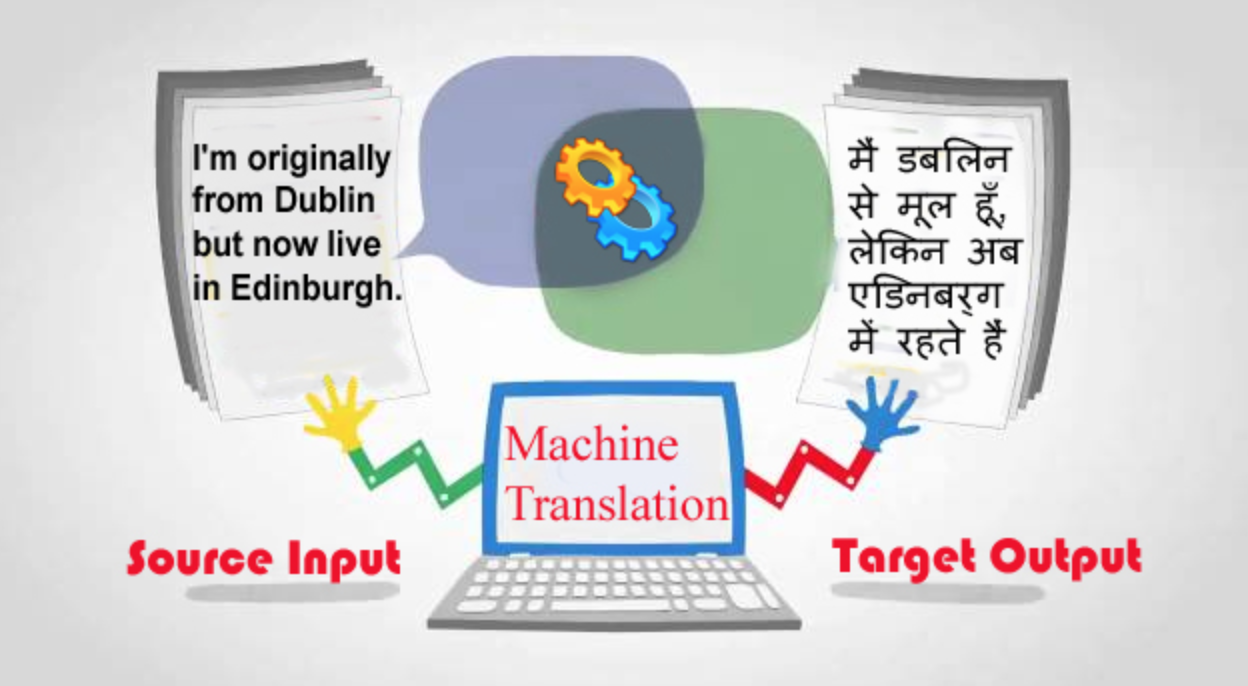
\includegraphics[width=\linewidth]{jiqifanyi.png}
      \caption{机器翻译}
  \end{subfigure}
  \begin{subfigure}[b]{0.4\linewidth}
    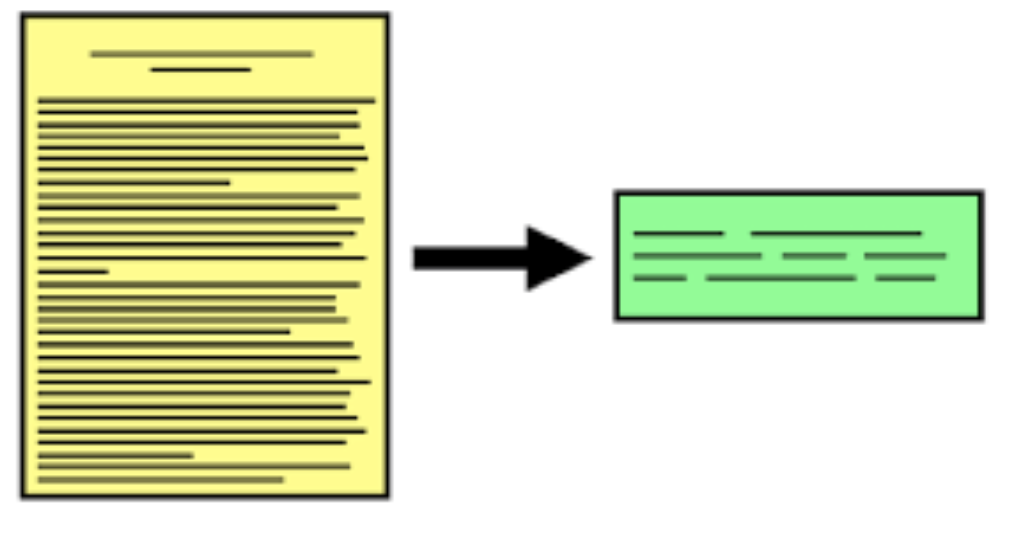
\includegraphics[width=\linewidth]{zidongchaiyao.png}
    \caption{自动摘要}
  \end{subfigure}
  \begin{subfigure}[b]{0.4\linewidth}
    
\includegraphics[width=\linewidth]{wendaxitong.png}
    \caption{问答系统}
  \end{subfigure}
  \begin{subfigure}[b]{0.4\linewidth}
      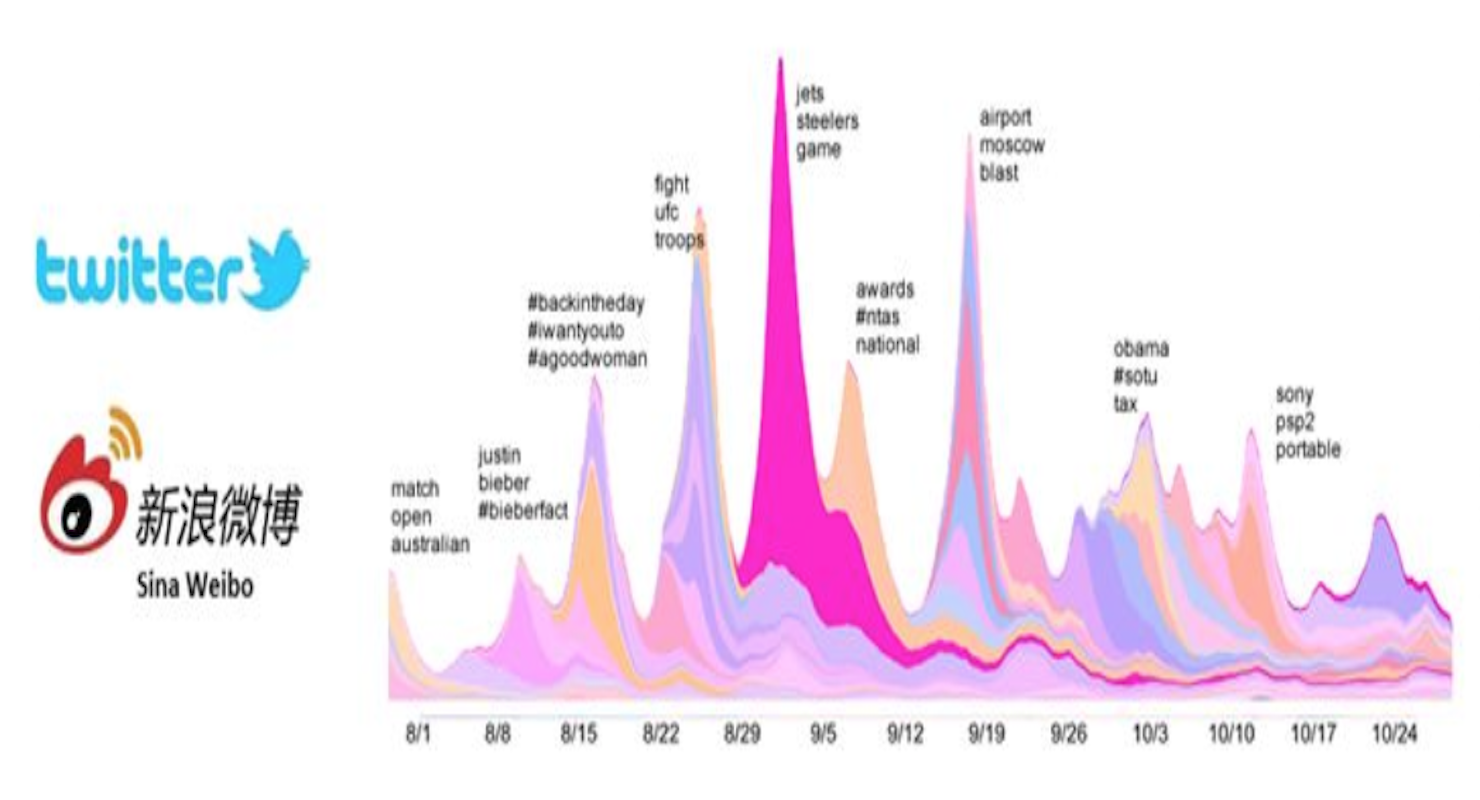
\includegraphics[width=\linewidth]{yuqingfenxi.png}
      \caption{舆情分析}
  \end{subfigure}
  \caption{文本理解的相关应用}
\end{figure}


所以对文本理解技术的研究必然可以推动NLP领域的发展,从而直接或间接推动这些应用的性能和实用性的提高,具有重要的研究意义和价值.

\section{文本理解研究的发展与现状}
\subsection{文本理解的早期发展}
文本内容理解的研究最早是从1954年的Georgetown大学的机器翻译系统\cite{SlocumMachine}研发开始的,
但是一开始是通过制定规则的语法入手,所以在系统构建上有很大的局限性,带来了翻译质量的低劣.
随着研究的深入,基于规则的思路面临越来越多的困难.
1966年,美国科学院下属的语言自动处理委员会(Automatic Language Processing Advisory Committee)
经过3年的研究发布了《语言与机器》的研究结论报告\cite{Pardelli2008From},
在这个报告中首次全面批判了机器翻译的研究可行性,并在报告中不建议政府继续支持机器翻译的研究.

此后一段时间对与机器翻译的研究跌倒了谷底,但是研究者仍然坚持对计算语言的理论进行研究,并产生了很多非常重要的研究成果,
比如在句法研究上1969年J.Earley提出的Earley句法分析算法\cite{Earley1970An}等,在语义分析上1966年C.J.Filmore提出的格语法等.


直到80年代后期,人们通过构建语料库,开始在自然语言处理中尝试统计学的方法,
尤其是把隐马尔可夫模型(Hidden Markov Model,HMM)从语音处理上引入到语言处理上,
这起到了推波助澜的作用,从而越来越多人开始通过在大规模语料库上运用统计机器学习方法,并量化的评价和比较各种评价方法的性能.


此后自然语言处理领域的研究从基于规则方法转到基于统计的方法.

\subsection{文本理解的研究现状}
Ruhi Sarikaya在2011年指出一个自然语言理解系统包括3个任务:
领域识别(domain detection),意图分类(intent determination)和属性抽取(slot filling)\cite{Tur2011Spoken},
它们是一个连续的过程,首先识别文本领域,之后对用户意图进行分类,最后实现属性抽取.


从技术上讲,领域识别和意图分类本质上是一个分类问题,通常使用传统的分类算法实现,
如2003年Haffner等人\cite{Haffner2003Optimizing,Chelba2003Speech,Chen2015Deriving}提出的支持向量机(Support Vector Machine,SVM)和
Chelba等人\cite{Chen2011Maximum}提出的最大熵算法(Maximum Entropy Classifier).
2014年Chen等人\cite{Ravuri2015Recurrent}提出也可以采用神经网络(Neural Network Classifier)来解决该问题.
而对于属性抽取则可以认为是一个序列标注问题,可以运用隐马尔可夫模型
和条件随机场(Conditional Random Field,CRF) 模型\cite{Pieraccini1992A,Wang2005Spoken}解决.

随着深度学习的发展,神经网络模型也被应用来处理领域识别和意图分类问题.
值得注意的是,Ravuri 和Stolcke 在2015年提出可采用循环神经网络(Recurrent Neural Network,RNN)来解决意图分类问题\cite{Sarikaya2011Deep,Tur2016Towards}.
而对于属性抽取,可通过深度学习来提取特征并与传统的CRF相结合\cite{Xu2014Convolutional}.Mesnil也尝试使用RNN进行序列标注以实现属性抽取\cite{Mesnil2013Investigation}.

循环神经网络经过实验证明在对序列化建模上效果显著,能够利用和记忆上下文信息,在几乎所有的NLP任务上都有很好的表现.
但是循环神经网络在反向传播求解的过程中会出现梯度消失和梯度爆炸的问题,所以对于长文本建模效果不佳.
后期提出的长短期记忆网络\cite{Graves2012Long}(Long Short-Term Memory,LSTM),通过在隐藏层设置3个“门”的结构,选择性的记忆和忘记,有效的解决了长文本建模的问题.
后来在此基础上有演化出许多改进的模型,比如树结构的长短期记忆网络\cite{Tai2015Improved}(Tree-LSTM),双向的长短期记忆网络\cite{Bahdanau2014Neural}(Bi-LSTM),
用来解决不同场景下的序列建模,如文本分类,中文分词,语义解析等.

目前以RNN为代表的深度学习模型已经成为了自然语言理解研究的主流方法.

但是这种方式的研究需要大规模的训练数据,并且将复杂的语言分析和理解过程简化成“黑盒子”,
模型中难以融合语言学知识,从而使整个模型缺乏很好的可解释性和鲁棒性.
这些被忽略的句子结构信息和其他语言学知识知识是可以用来辅助提升模型的,比如对于训练语料库中未出现的句子的词序列标注\cite{Deoras2013Deep}.

Liu与Chen分别在2013年\cite{Liu2014Query}和2015年\cite{Chen2015Matrix},提出通过对句子中语言学知识进行编码可以提升文本理解能力,提取出来的句法结构特征和语义依存信息能够提高模型的理解力,并在多个领域均取得了更好的文本理解效果.
但是目前已有的融合语言学知识和深度学习的方案,都是将语言学知识作为额外的特征输入到神经网络中,然后训练模型进行词序列标注.这样同样会产生一些局限性,包括较差的归纳性和错误信息会在网络中持续传播.

所以NLP未来发展的重要方向将会是如何有效的引入语言本身的语言学知识,来使模型具备好的可解释性和鲁棒性.

\section{论文主要工作}
本文围绕研究将语言中的先验知识与深度学习模型进行有机融合,提出了融合依存句法结构的深度神经网络,并基于文本分类任务,研究融合模型的效果.
具体来说,本文的研究内容有下面几个方向.

(1)通过斯坦福句法分析工具,构建文本的依存句法树,解析出子文本结构.

(2)研究和复现传统的RNN、LSTM等深度神经网络模型,并在LSTM模型的基础上融合依存句法信息,构建融合模型.

(3)研究了融合模型在不同规模数据集上表现和对通过可视化文本重要程度研究模型的可解释性.

(3)研究了文本结构的Attention机制和融合方式对模型效果的影响,并选择最佳的Attention和融合方式.

\section{论文结构安排}
本论文总共分为五个章节,每个章节的内容概括如下:

(1)第一章为绪论,首先介绍了文本理解的研究背景及意义,然后介绍了该领域的研究发展和 现状,并且简单描述了本文的研究内容,最后给出了全文的结构安排.

(2)第二章为基于深度学习的文本理解,
包括Word Embedding的文本表示方法,RNN、LSTM深度学习模型的介绍
以及基于深度学习的依存句法分析.

(3)第三章为融合句法结构树的深度神经网络模型,详
细介绍了融合模型的整体架构和每个模块的细节.

(4)第四章为实验部分,基于语料库AGNews,设计了融合模型和其他传统模型的对照实验,
并对不同的数据集、Attention方式、融合方式进行了深入的实验和分析.

(5)第五章为结论与展望,对本文主要工作进行了总结,对存在的不足进行了展望.


\chapter{基于深度学习的文本理解方法}
\section{文本的词向量表示方法}
自然语言处理领域最小的单元就是词语,通过词语构成句子,再有句子构成篇章.
所以为了让计算机能够处理文本首要任务就是对词语进行表示.
好的文本表示能够更加真是的反应文本的内容,对于不同的内容有更好的区分能力.

现在主流的表示方法是基于词向量(word embedding)的文本表示.
通过词向量可以讲词转化成稠密向量,对于相似的词,对应的词向量也相近.
这种表示方法又可以分为独热表示(one-hot representation)和分布式表示(distributed representation).

\subsection{独热表示}
用词向量表示文本,独热表示是一种最直接也是最简单的表示方法.
具体来说,每个词都表示成一个$n$维的向量,这里$n$为语料库中词表的大小.
假设某个单词在词表中的位置是$k$,那么这个单词的词向量只有位置$k$是1,
其他位置均是0.

比如有一个句子“我喜欢音乐,尤其是摇滚和嘻哈.”
如果整个语料库中就仅有这一个句子,这个句子分词后有8个不重复的单词,所以每个单词都可以表示为一个8维的向量,如下表所示.

\begin{table}[h!]
  \centering
  \begin{tabular}{cccccccc}
    \toprule
    \textbf{我} & \textbf{喜欢} & \textbf{音乐} & \textbf{尤其} & \textbf{是} & \textbf{摇滚}  & \textbf{和} & \textbf{嘻哈}  \\
    \midrule
    1 & 0 & 0 & 0 & 0 & 0 & 0 & 0 \\
    0 & 1 & 0 & 0 & 0 & 0 & 0 & 0 \\
    0 & 0 & 1 & 0 & 0 & 0 & 0 & 0 \\
    0 & 0 & 0 & 1 & 0 & 0 & 0 & 0 \\
    0 & 0 & 0 & 0 & 1 & 0 & 0 & 0 \\
    0 & 0 & 0 & 0 & 0 & 1 & 0 & 0 \\
    0 & 0 & 0 & 0 & 0 & 0 & 1 & 0 \\
    0 & 0 & 0 & 0 & 0 & 0 & 0 & 1 \\
    \bottomrule
  \end{tabular}
  \caption{8维独热词向量表示}\label{table:3t1}
\end{table}

通过稀疏的方式存储这种表示会非常的简单.
也就是给每个单词分配一个数字ID,如示例中的音乐为2,摇滚乐5(从0开始).
所以在编程中构建一个ID-单词的哈希表,这种方案效率是O(1),结合成熟的
SVM、CRF、最大熵等机器学习算法就能在很多主流的NLP任务上取得很好的效果了.

然而这种方案有个非常的大弊端,也就是所谓的“词汇鸿沟”:
任意两个词的词向量之间都是正交,也就是说明词与词之间是彼此独立的.
如果仅仅通过词向量无法看出两个词语义上的关系.比如例子中的音乐和摇滚在语义上是相关的,但这种相关性无法从词向量上体现出来.

\subsection{分布式表示}
为了解决独热法无法体现语义的问题,Hinton等人\cite{Rumelhart1986Learning}在1986年提出了一种新的表示方法:Distributed representation,也就是“分布式表示”.

这种表示的基本思想是,构建一个词向量训练模型,通过训练把每个词表示成一个$N$维的向量,其中$N$是一个可调节的参数.
这样两个词向量之间的距离,比如欧式距离,cosine相似程度就可以用来衡量两个词之间的语义关系.

2003年Bengio\cite{Turian2010Word}提出了一种经典的三层的神经网络“输入层-隐层-输出层”模型来训练词向量.
其核心思想是:一个给定单词的意思是由它的上下文确定的.
通过将被预测词的前$n$个词连接后作为神经网络的输入项,最后通过softmax层计算得到改词的词向量表示.
这种训练得到的词向量有很强的语义相关,
例如,$V(\mbox{中国})-V(\mbox{北京})+V(\mbox{东京}) = V(\mbox{日本})$,
类似的,$V(\mbox{王妃})-V(\mbox{女人})+V(\mbox{男人})=V(\mbox{国王})$.
这样的结果非常振奋人心,但是这个算法对计算要求很高,训练效率较低.

2013年Google的Mikolov等人提出了Word2vec工具包\cite{Mikolov2013Distributed},里面包括了两种新的词向量模型:
CBOW(continuous bag of words)模型:给定上下文词,预测是否是中心词
和skip-gram模型:给定中间词,预测是否是上下文词.
Word2Vec真正出名的是因为模型的高效性,模型中通过引入负样本(negative sample)和层间softmax(hierarchical softmax)
两种方案大幅度提升了训练效率,在一个单机上就可以完成每天千亿级别词向量的训练.

\begin{figure}[h!]
  \centering
  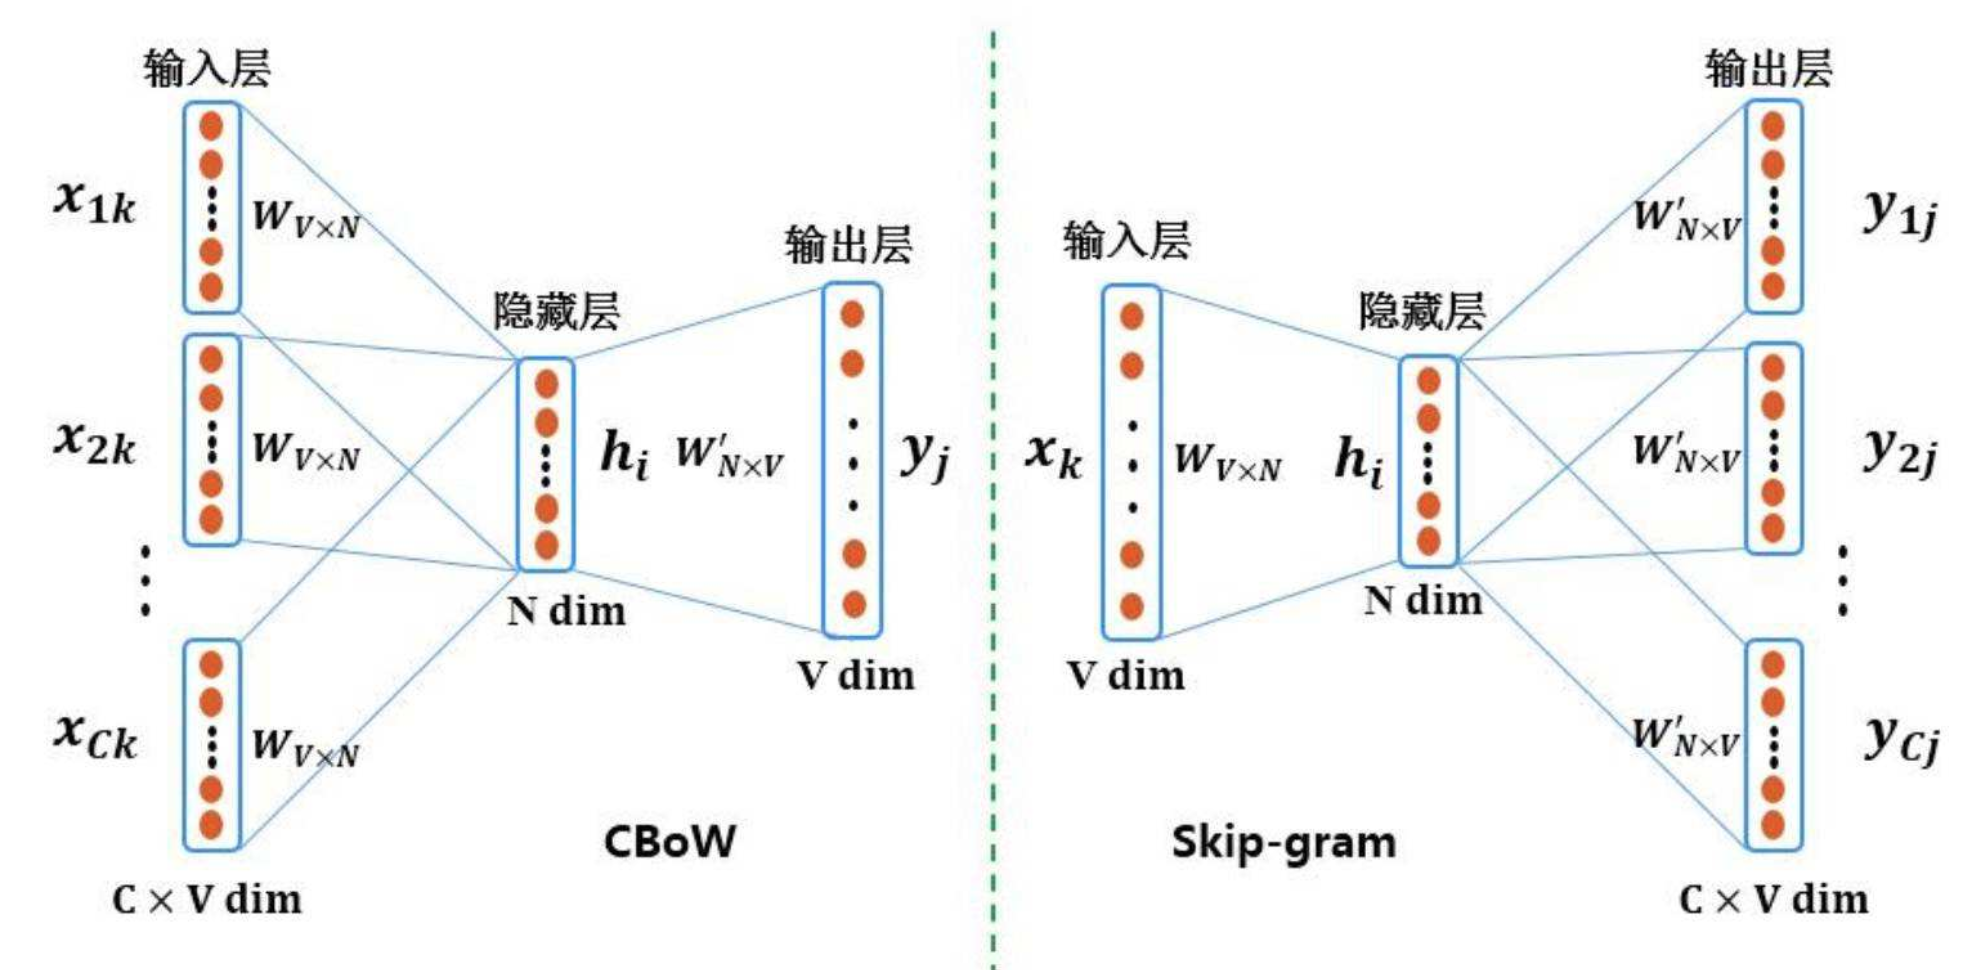
\includegraphics[width=0.6\linewidth]{CBOW-skip-gram.png}
  \caption{CBOW和skip-grams模型图示}
\end{figure}

具体来说,遍历文本中的每一个位置,包括一个中心词$c$和上下文单词$o$,通过词向量的$c$与$o$的相似度来计算$o$是$c$上下文的可能性,
通过调整词向量使得全局可能性达到最大.对于每个位置$t$,中心单词为$w_{t}$,窗口大小为$m$,那么全局可能性为:

\begin{equation}
  L(\theta) = \prod_{t=1}^{T} \prod_{-m \le j \le m ;j \neq m} P(w_{t+j}|w_{t},\theta)
\end{equation}

所以损失函数可以写成:
\begin{equation}
  J(\theta) = -\frac{1}{T}logL(\theta) = -\frac{1}{T} \sum_{t=1}^{T} \sum_{-m \le j \le m ;j \neq m} log P(w_{t+j}|w_{t},\theta)
\end{equation}

其中概率$P$通过$softmax$函数计算,采用梯度下降算法训练参数.

\subsection{GloVe模型}
Word2vec是基于局部上下文进行词向量训练的,所以并没有考虑到全局的信息.
2014年斯坦福大学的Jeffrey Penninngton等人\cite{Pennington2014Glove}提出了无监督学习的Glove(Global Vectors for Word Representation)模型.

其主要思想是以某个词的上下文窗口遍历整个语料库,统计窗口中词与词共同出现的次数,得倒整个语料库的词共现矩阵,
最后利用矩阵中的非零元素训练词向量.

设整个词共现矩阵为$X$,那么$X_{i}$为单词$w_{i}$上下文中所有出现词的总和,也就是矩阵第$i$行的和
,$X_{i,j}$表示单词$w_{i}$上下文中$w_{j}$出现的次数.那么单词$w_{j}$在$w_{i}$上下文中的概率为:

\begin{equation}
  P_{i,j} = P(w_{j}|w_{i}) = \frac{X_{i,j}}{X_{i}}
\end{equation}

两个词的共现概率就可以体现两个词的相关性.给定一个词$w_{k}$,通过计算$p_{ki}$ 与$p_{kj}$的比值,
来判断$w_{i}$和$w_{j}$哪一个与$w_{k}$更相关,如果比值大于1,则是单词$w_{i}$,反之就是单词$w_{j}$.
模型中词与词之间共现概率的比值可以最终转换成需要优化的目标函数:

\begin{equation}
  J = \sum_{i,j}^{N}f(X_{i,j})(v_{i}^{T}v_{j}+b_{i}+b_{j}-log(X_{i,j}))^2
\end{equation}

上式中的$v_{i}$,$v_{j}$表示单词$i$和$j$的词向量,
$b_{i}$,$b_{j}$是偏差项,是两个标量.
$N$是词汇表的大小,共现矩阵维度为$N*N$,$f$是权重函数,需要满足一定的非递减性,
来保证对低频词共现组合不会赋值很大,所以一般$f(X_{i,j})$定义为:

\begin{equation}
  f(x) = 
  \left\{
    \begin{array}{lr}
      (x/x_{max})^{\alpha}, & x<x_{max} \\
      1, & x \ge x_{max} 
    \end{array}
    \right.
\end{equation}

其中,$\alpha$一般取$0.75$,$x_{max}$则根据语料库的实际情况而定.


\section{NLP领域的深度学习模型}
神经网络模型具备强大的学习能力和拟合能力,在图像、音频,NLP等诸多领域取得了非常好的效果.
NLP领域应用最为广泛的深度学习模型就是循环神经网络RNN和长短期记忆网络LSTM.

\subsection{循环神经网络}
传统的神经网络是对一个时间点进行建模,所以不能对时序数据建模.比如对于一个文本进行分类,
传统神经网络只能对一个单词进行建模,而不能对整个句子进行建模.
而循环神经网络RNN的出现很好的解决了对序列数据建模的问题.

循环神经网络,顾名思义,就是当前节点的输出还会作为下一个节点的输入.
所以神经网络中的隐藏层节点不是彼此独立的,而是相互之间有连接的,
这样网络就会对整个序列的信息进行记忆,并体现到每个节点的计算中.
下图是一个典型的RNN结构图:

\begin{figure}[h!]
  \centering
  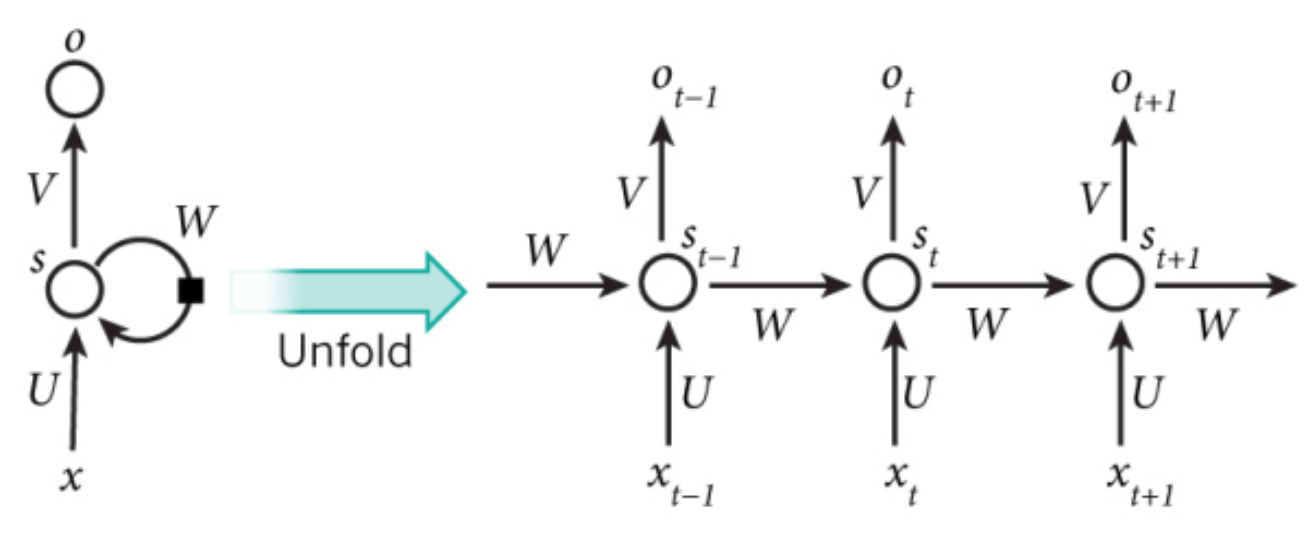
\includegraphics[width=0.6\linewidth]{RNN.png}
  \caption{RNN结构图}
\end{figure}

如图所示,可以将循环神经网络按照序列展开成一个全连接的神经网络.
比如对以一个仅有3个单词构成的句子,那么就可以展开形成一个3层神经网络,网络中的每一个就表示一个单词.
一般的对于第$t$步,$x_{t}$表示输入,$o_{t}$表示输出.
$s_{t}$表示隐藏层的状态,这是$x_{t}$和$o_{t-1}$计算而来的,是网络中的记忆模块.

\begin{equation}
  \left\{
  \begin{array}{l}
    s_{t} = f(U*x_{t}+W*s_{t-1}) \\
    o_{t} = softmax(V*s_{t})
  \end{array}
  \right.
\end{equation}

上式中的$f$表示非线性的激活函数,如$tanh$,$ReLU$.
对于RNN来说整个网络中只有参数$U$,$V$,$W$,所以层之间的参数是共享的,
也正是如此,这些参数表征了整个序列,并且也使得网路中要学习的参数不会随着序列长度增加而增加,提高了学习效率.
对于RNN的训练同样是误差反向传播算法.

RNN有4种常见的架构,1 to N、N to 1、N to N和N to M,这4种架构基本可以满足常见的NLP应用.

\begin{figure}[h!]
  \centering
  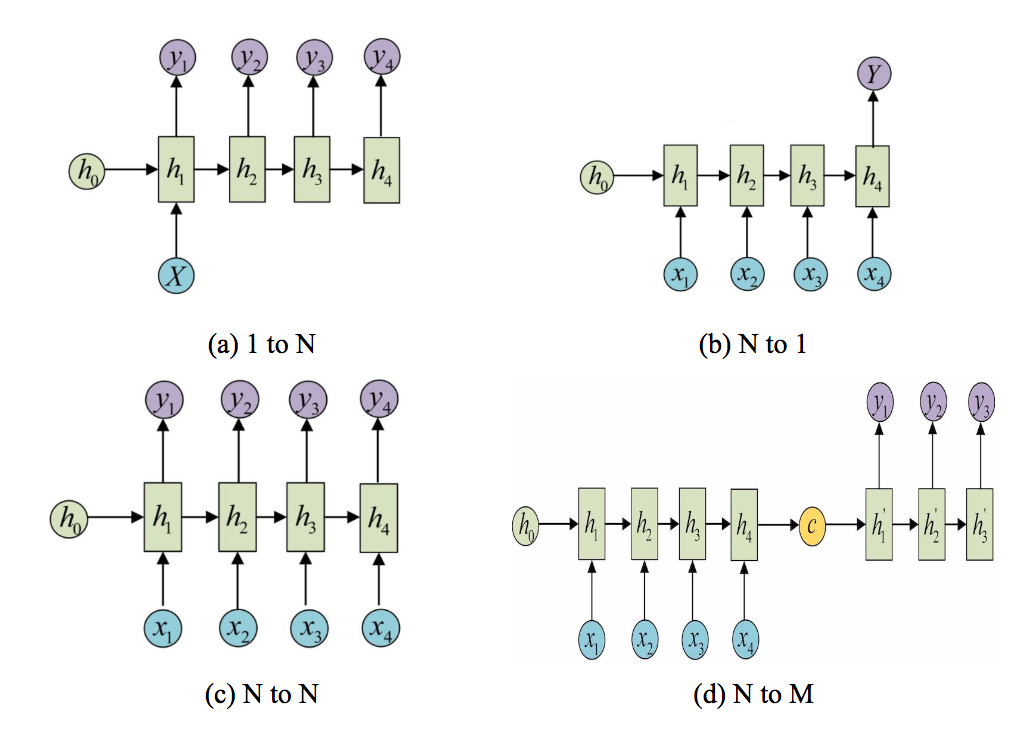
\includegraphics[width=0.65\linewidth]{4zhongjiagou.png}
  \caption{RNN4种架构}
\end{figure}

% \begin{figure}[h!]
%   \centering 
%   \begin{subfigure}[b]{0.4\linewidth}
%     \includegraphics[width=\linewidth]{1ton.png}
%     \caption{1 to N}
%   \end{subfigure}
%   \begin{subfigure}[b]{0.4\linewidth}
%     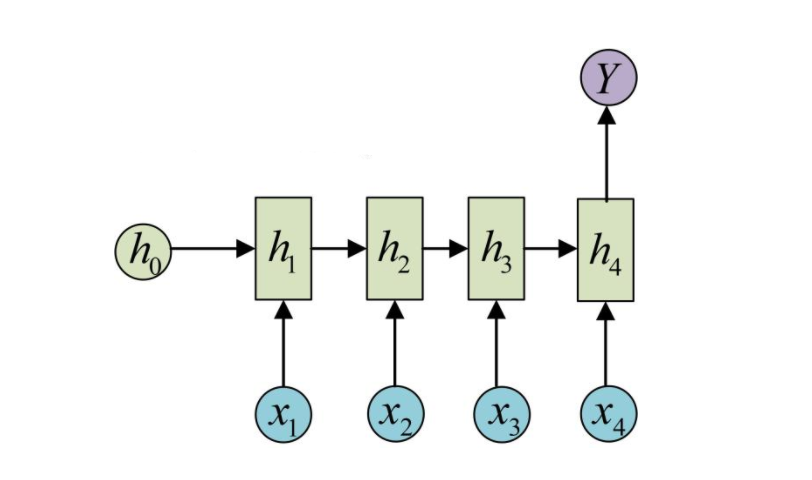
\includegraphics[width=\linewidth]{nto1.png}
%     \caption{N to 1}
%   \end{subfigure}
%   \begin{subfigure}[b]{0.4\linewidth}
%     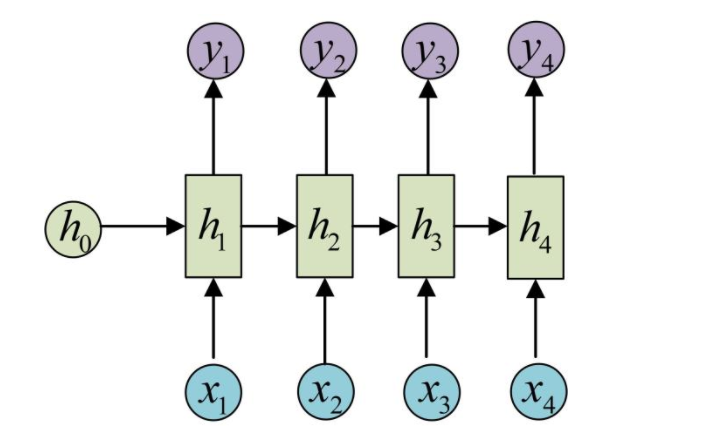
\includegraphics[width=\linewidth]{nton.png}
%       \caption{N to N}
%   \end{subfigure}
%   \begin{subfigure}[b]{0.4\linewidth}
%     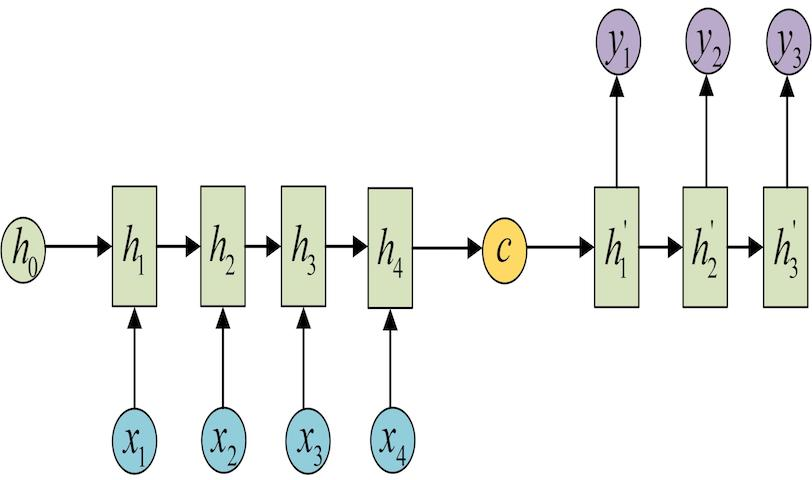
\includegraphics[width=\linewidth]{ntom.jpg}
%     \caption{N to M}
%   \end{subfigure}
%   \caption{RNN的4种常见的架构}
% \end{figure}


(1)1 to N:输入是一个值,输出是一个序列.比如图片标注,输出的X是图像的特征,而输出的y序列是一段句子,或者输入类别x,输出的y是该类别的一串文字.

(2)N to 1:输入是一个序列,输出是一个单独的值.这种架构最典型的应用就是分类问题,
比如输入是一段音频、视频或者文本,输入是属于哪一个类别.


(3)N to N:这种架构输入和输出均是一个序列的形式,并且长度相等.
最简单的就是输入一个单词,生成一个单词,也就是CharRNN,通过扩展
就是用来自动作诗,谱曲甚至写代码.

(4)N to M:这种架构输入输出同样是一个序列的形式,但是长度可以不相等.
所以可以称为Seq2Seq模型,也可以认为是编码-解码模型.这种模型相对于NtoN
更加的一般和实用,因为实际应用中大部分情况输入输出序列是不相等,比如机器翻译就是这类的典型应用.

但是RNN在对长序列建模上会有严重的问题,在反向传播的时候对于距离较远的节点会进行
雅可比矩阵连乘,这样如果特征值是小于一幂次以后趋向于0,也就造成了“梯度消失”,而如果大于1,那么幂次以后就会趋向于无穷大,
造成“梯度爆炸”.

\subsection{长短期记忆网络}
为了解决RNN对长序列建模的困难,研究人员提出了许多解决办法,例如ESN(Echo State Network),
增加有漏单元(Leaky Units)等.
其中最成功应用最广泛的就是门限RNN(Gated RNN),而长短期记忆网络LSTM就是门限RNN中最著名的一种.

\begin{figure}[h!]
  \centering
  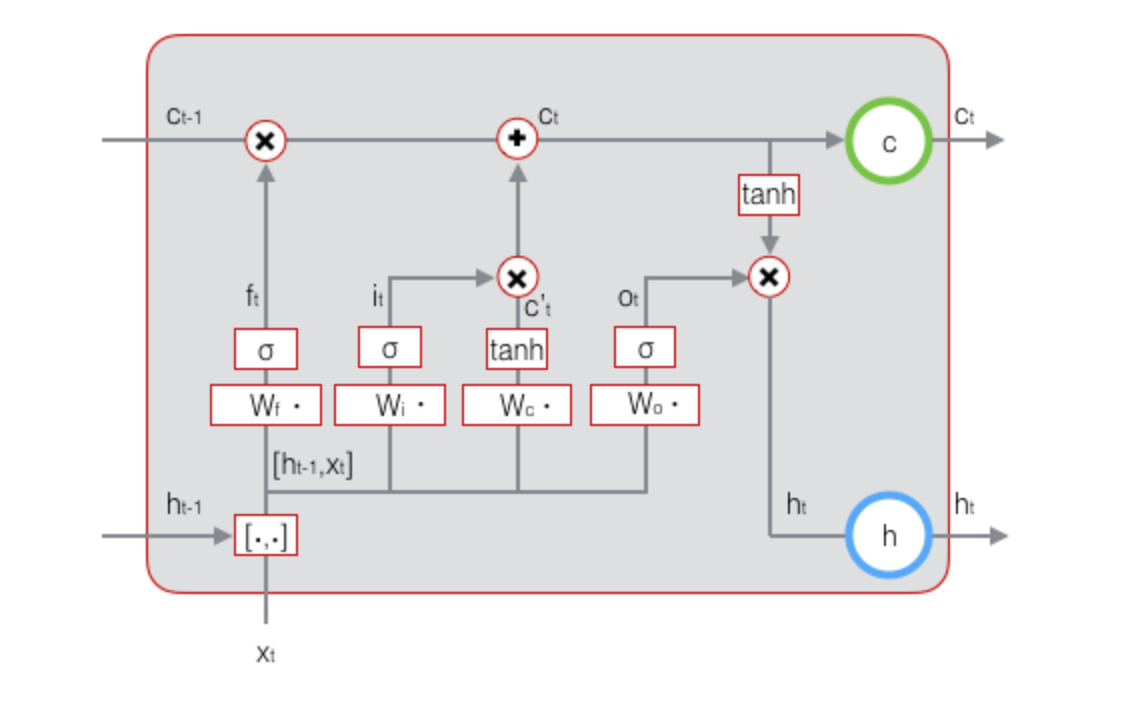
\includegraphics[width=0.6\linewidth]{LSTM.png}
  \caption{LSTM模型}
\end{figure}

如上图所示,LSTM一个单元通过输入门、遗忘门、输出门三个门来控制信息的流动,
其中输入门控制信息的流入,
遗忘门负责丢弃记忆细胞中的无用信息,
最后输出门控制信息的输出.
还有一个记忆细胞负责储存先前的信息和产生下一个输出.
对应的公式为:

\begin{equation}
  \left\{
  \begin{array}{l}
   i_{t} = \sigma(W^{xi}x_{t}+W^{hi}h_{t-1}+b_{i}) \\ 
   o_{t} = \sigma(W^{xo}x_{t}+W^{ho}h_{t-1}+b_{o}) \\ 
   f_{t} = \sigma(W^{xf}x_{t}+W^{hf}h_{t-1}+b_{f}) \\ 
   \widetilde{c}_{t} = \sigma(W^{xc}x_{t}+W^{hc}h_{t-1}+b_{c}) \\
   c_{t} = f_{t} \odot c_{t-1} + i_{t} \odot \widetilde{c}_{t} \\
   h_{t} = o_{t} \odot c_{t}
  \end{array}
  \right.
\end{equation}

式子中的$W$和$b$是模型参数,$i_{t}$,$o_{t}$,$f_{t}$对应$t$时刻的输入门,输出门和遗忘门,
$\widetilde{c}_{t}$,表示遗忘细胞更新量,由输入门,遗忘门,上一个时刻的记忆细胞,和当前记忆细胞的更新量,共同计算当前的记忆细胞值.
然后通过当前的记忆细胞和输出门计算当前时刻的隐层输出$h_{t}$.

显然LSTM单元可以无缝的替换传统的RNN单元,
所以LSTM也有4种架构,
采用RNN模型的应用几乎都可以很方便的替换成LSTM模型.
但是这类模型,并没有运用到语言本身句法结构中的信息,模型处于黑盒之中,缺乏必要的直观性和鲁棒性.

\section{基于深度学习的依存句法分析}
\subsection{依存句法的概念}
1960年基于当时机器翻译的特点,美国语言学家D.GHays提出了依存句法的概念\cite{Hays1960Grouping}.
这里的“依存”,表示两个词之间的上下级关系,是一种有方向、支配与被支配的关系.
在依存结构图中用带有方向的弧表示了两个词之间的支配和被支配关系,也指明了这两个词在语义层次的搭配关系.
比如“I shot an elephant in my pajamas.”的依存句法结构如下图所示.

\begin{figure}[h!]
  \centering
  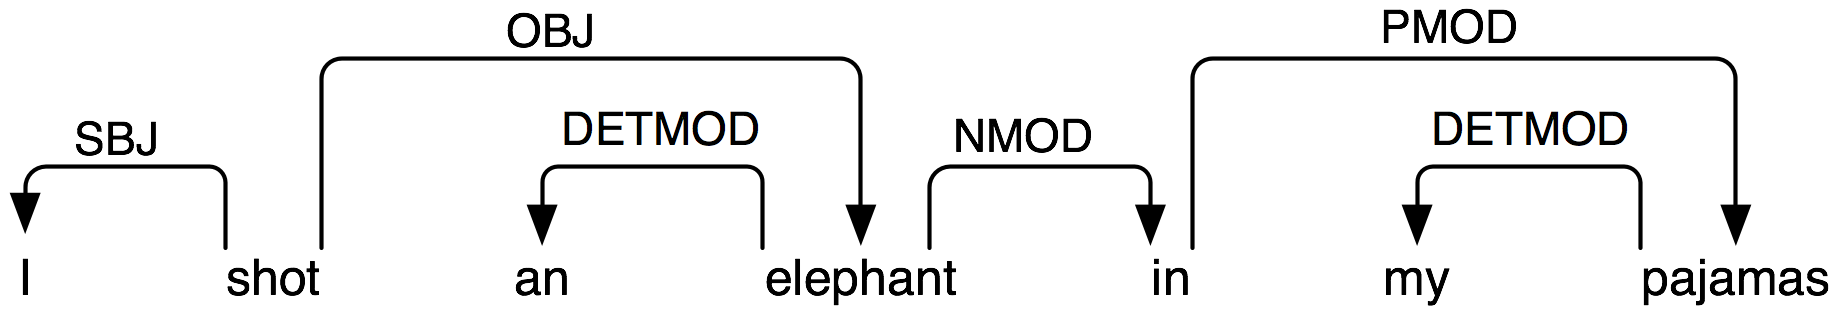
\includegraphics[width=0.7\linewidth]{yicunjufa.png}
  \caption{依存句法示意图}
\end{figure}

随着句法理论的发展计算机语言学家罗宾森总结了依存语法的五条定理:

(1)一个句子中存在一个根节点(Root),这个节点是不依赖任何其他任何节点的.

(2)其它成分直接依存于某一成分.

(3)任何一个节点均只能依存于一个成分.

(4)如果A成分直接依存于B成分,而C成分在句中位于A和B之间,
那么C可能直接依存B,或者间接依存于A和B中间的某个部分.

(5)中心词两边的成分不存在依存关系.

所以一个句法结构中只有一个根节点,并且可以用树来表示整个结构,如下图所示,
树中节点直接依存其父亲节点,
也就是树中的父节点支配子节点.

\begin{figure}[h!]
  \centering
  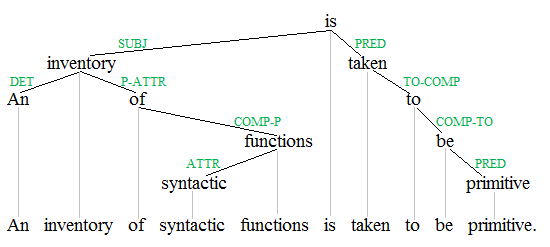
\includegraphics[width=0.6\linewidth]{yicunjufashu.png}
  \caption{依存句法树示意图,隐去了Root节点}
\end{figure}

句子成分中的支配和被支配的依存关系具有广泛的普遍性,
在词汇,短语,篇章等各级别的语言单位之间都存在.
所以依存句法反应了句子内部的词与词之间的语义修饰关系,
并且这种关系和词与词之间的位置关系是没有联系的,
所以直接体现了句子中蕴含的语言学知识,具有很大的利用价值.

\subsection{Stanford Parser}
Stanford Parser 是由斯坦福大学自然语言处理小组开发的开源句法分析器.
最新版的分析器是基于深度神经网络的,由Danqi在2014年提出并实现\cite{The}.

整个模型具体来说,首先先把每个单词表示成一个$d$维的向量$e_{i}^{w} \in \mathbb{R}$,
所以整个词向量矩阵就是$E^{w} \in \mathbb{R}^{d*N_{w}}$,
这里的$N_{w}$表示词典的大小.
同时吧POS标签和弧形标签映射成一个$d$维的向量,
$e^{t}_{i}$,$e^{l}_{j}$分别表示第$i$个POS标签和第$j$个弧标签,
所以整体上$E^{t} \in \mathbb{R}^{d*N_{t}}$,$E^{l} \in \mathbb{R}^{d*N_{l}}$,
这里的$N_{t}$表示POS标签数量,$N_{l}$表示弧度标签数量.
通过建立一个标准的神经网络,有一个隐藏层,把$(word,POS,arc)$的组合
作为神经网络的输入,并且把输入的3次方映射成隐藏层,最后通过一个softmax函数.
网络的结构如下图所示.


\begin{figure}[h!]
  \centering
  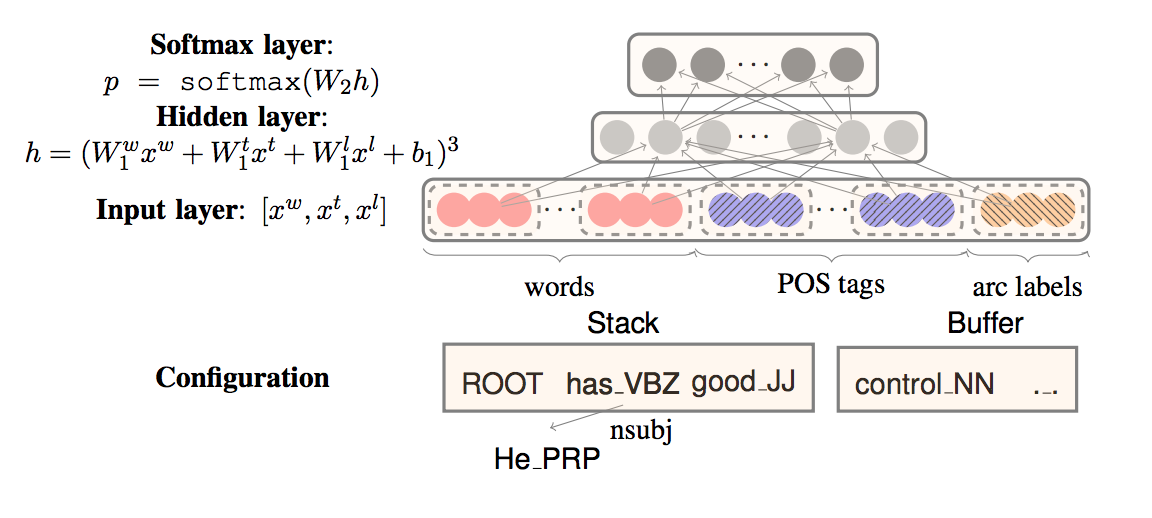
\includegraphics[width=0.85\linewidth]{sitanfujufafenximoxing.png}
  \caption{斯坦福句法分析模型}
\end{figure}

这个模型提出后,在CoNLL依存句法数据集上一直稳居第一名.具体来说Stanford parser有下面几大优点:

(1)通过全面可靠的语料库进行训练,并且已经开发了多个语言,包括英语、中文、葡萄牙语在内的10多种语言.

(2)是一个高效的分析器,支持多种形式的输出,包括结构的文本输出和树形结构的输出.

(3)分析器内置了众多的NLP工具,包括分词、词法标注等.

在使用上Stanford Parser是给予Java语言开发的,也提供了多个语言的变成接口,
并且还可以以服务的方式运行,提供API调用.
目前已经集成进了Stanford CoreNLP工具包中.



\chapter{融合句法结构的深度神经网络模型}
本章节详细介绍提出的融合句法结构的深度神经网络模型(下文简称:融合模型).
该模型是将蕴含语言学知识的依存句法结构信息融合到传统的LSTM模型中,
以提升文本理解的效果.
\section{模型设计}
这个部分将说明如何对文本内容和语言学知识进行向量化的编码,
并着重说明融合模型的架构,详细说明各个模块的运作方式.
\subsection{词向量设计}
有两个词向量的设计工作,第一是将文本的向量化,第二是将依存句法结构向量化.

对于第一个文本的向量化,可以采用先前介绍的Glove模型来训练词向量,
或者直接从官网https://nlp.stanford.edu/projects/glove/上下载已经训练好的词向量.
这些词向量是通过英文维基百科训练的,维度有多种,包括50,100,200,300维等.
设每个单词表示成一个$d$维的向量$e_{i}^{w} \in \mathbb{R}$,所以一段文本可以表示为
$E^{w} \in \mathbb{R}^{d \times N_{w}}$,其中$N_{w}$表示这段文本的长度.

对于第二个依存句法结构的向量化,首先通过斯坦福句法分析工具包生成依存句法树.
这样可以获得依存句法树根节点到叶子节点的形成的子结构.

比如,对于句子“show me the flights from seattle to san francisco.”
可以获得的子结构如下图所示.

\begin{figure}[h!]
  \centering
  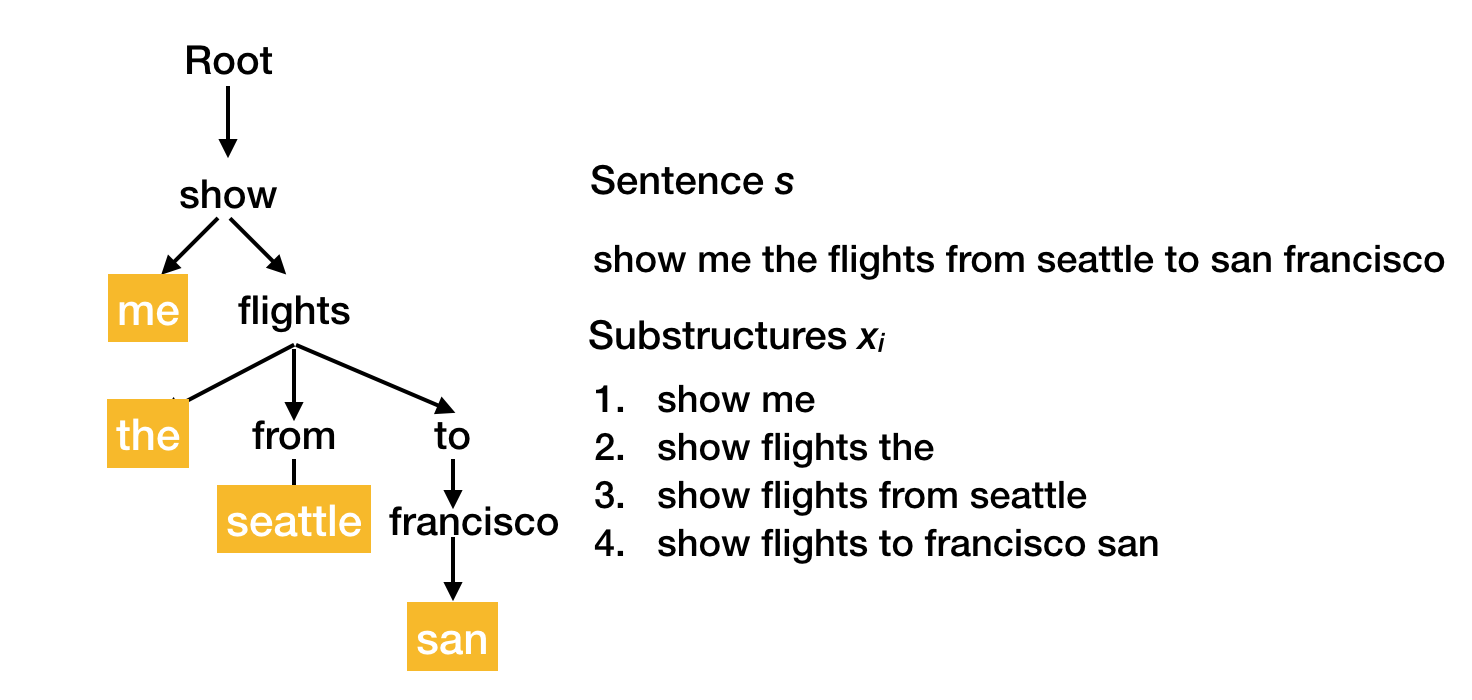
\includegraphics[width=0.8\linewidth]{yicunjufashujuli.png}
  \caption{根据依存句法树获得子结构}
\end{figure}

这样上面图中的依存句法结构就可以通过这4个子串$x_{1},x_{2},x_{3},x_{4}$来表示,
事实上仅仅通过这4个子串就可以反过来推导出依存句法树,
所以依存句法树和其从根节点到叶子节点的子串是相互唯一确定的.

下面对这4个子串进行向量化,每个单词依然表示成一个$d$维的向量,
那么一个子串$x_{i}$就可以表示为$E_{x_{i}} \in \mathbb{R}^{d*N_{x_{i}}}$,
这里$N_{x_{i}}$表示子串$x_{i}$的单词个数.
值得注意的是所有子串的总数一定是小于文本中所有单词数量的,
因为子串是根据叶子节点获得的,非叶子节点就没有对应的子串,
这样也可以减少模型中的重复信息.

最后还需要说明一下,如何根据依存句法树中获得所有从根节点到叶子结点的子串,
事实上可以通过一个简单的递归算法解决,具体如下.

\begin{table}[h!]
  \centering
  \begin{tabular}{l}
    \toprule
    \textbf{递归获取依存句法树子串算法描述} \\
    \midrule
    (1)输入: 依存句法树Tree \\
    (2) 定义所有子串的列表$all\_substructures$,路径字符串$path$ \\
    (3) 定义递归函数$walk(node,path)$,$node$为当前节点 \\
    (3.1) 路径字符串加上当前节点的值 $path = path + node.value$ \\
    (3.2) 判断当前节点是不是叶子结点,如果是转到(3.3),如果不是转到(3.4)\\
    (3.3) 所有子串的列表加上当前的路径字符串,$all\_substructures.append(path)$ \\
    (3.4) 对该节点所有的子节点递归调用,$walk(node.childnode,path)$ \\
    (4)调用 $walk(Tree.root\_node,path)$ \\
    (5)输出所有子串的列表$all\_substructures$ \\
    \bottomrule
  \end{tabular}
  \caption{递归获取依存句法树子串算法描述}
\end{table}
通过上面的算法输入依存句法树就可以获取所有的子结构.

\subsection{模型架构}
融合句法结构的深度神经网络模型的整体架构如下图所示:
\begin{figure}[h!]
  \centering
  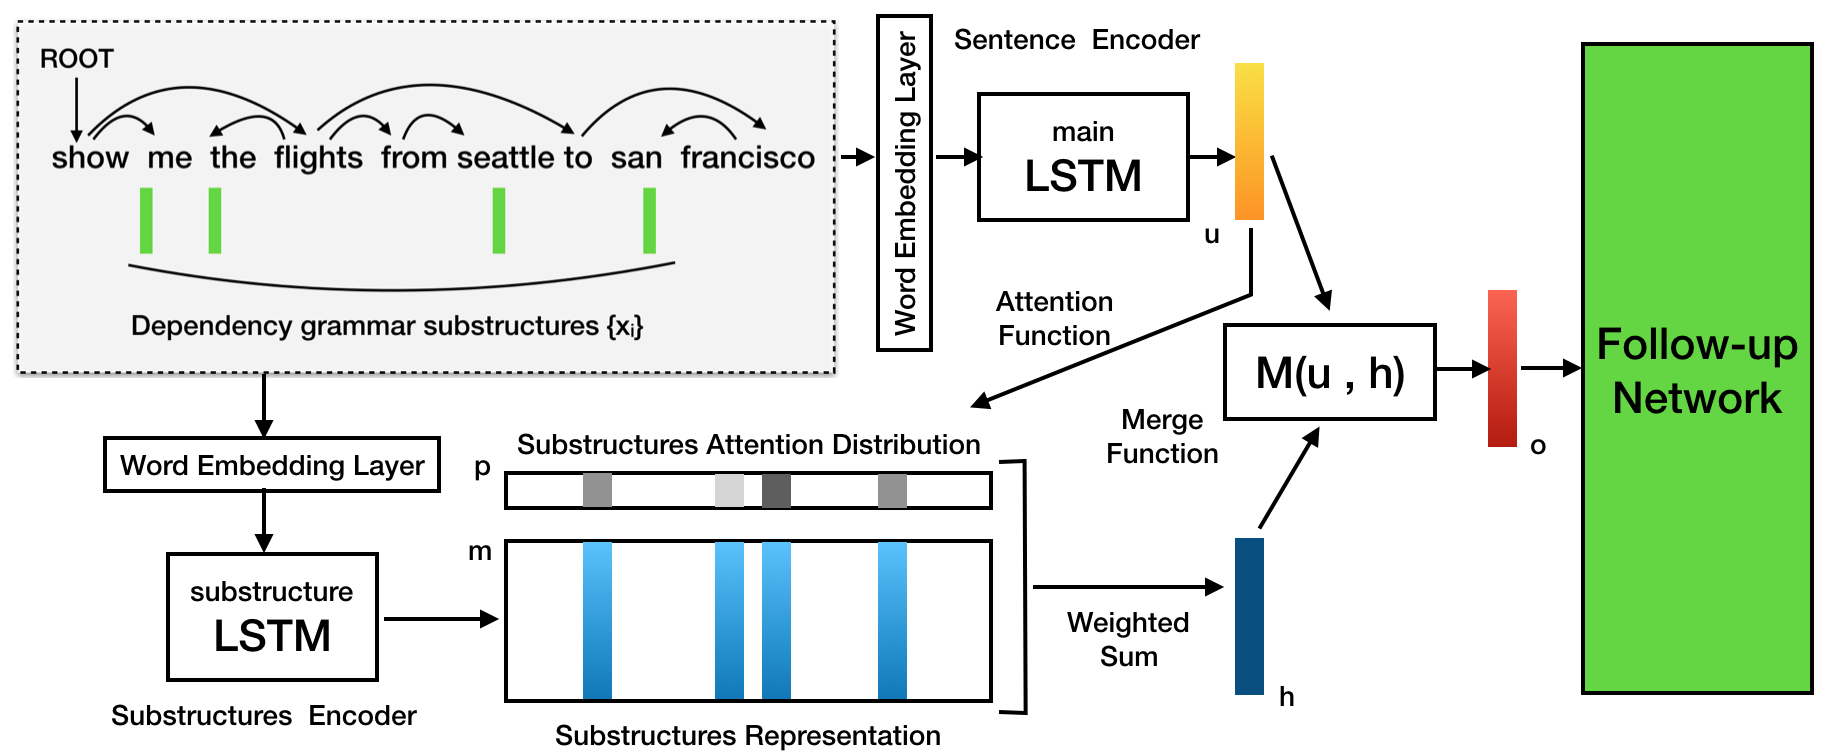
\includegraphics[width=0.95\linewidth]{model.png}
  \caption{融合句法结构的深度神经网络模型}
\end{figure}

整个模型图示从左向右看子结构句子和主文本句子分别通过两个LSTM模型,
将子结构输出的结果加权平均后与主文本句子的输出结果相融合,
得到一个最终的融合表示,最后将这个表示送入后续的神经网络中,
完成文本分类、机器翻译等文本理解的应用.下面对具体的阐述模型中的几个细节.

(1) 这里的词嵌入层直接采用Glove的词向量,只需要将单词与词向量进行一一映射即可.
词向量的维度$d$是模型的超参数.

(2)LSTM模块采用单层经典的LSTM模型即可,事实上在本模型中,LSTM可以看成一个编码器,
我们只取LSTM的最后一个隐藏层节点,因为LSTM具有记忆的功能,
所以最后一个节点可以认为是对整个输入文本的编码.
所以$x_{i}$被编码成$m_{i}$,整个文本句子$s$被编码成$u$,
其中$m_{i} \in \mathbb{R}^{H_{sub}}$ ,$H_{sub}$为子结构LSTM隐藏层节点个数,
$u \in \mathbb{R}^{H_{main}}$,$H_{main}$为主LSTM隐藏层节点个数.

\begin{equation}
\left\{
  \begin{array}{l}
   m_{i} = LSTM_{sub}(x_{i}) \\ 
   u = LSTM_{main}(s) \\ 
  \end{array}
  \right.
\end{equation}

LSTM的内部推倒可以见2.2.2小节,
下面通过一个图示来说明通过LSTM模型的过程,
一个子结构句子“show me the”通过LSTM,
并将最后一个隐藏层输出作为编码结果$m$.

\begin{figure}[h!]
  \centering
  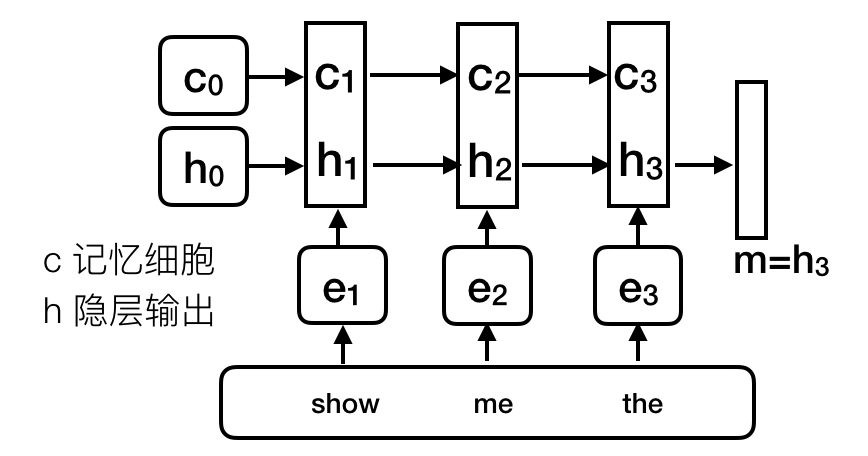
\includegraphics[width=0.5\linewidth]{LSTMjuti.png}
  \caption{$x$通过LSTM编码得到$m$}
\end{figure}

(3)
通过Attention函数来计算整个句子的编码$u$和每一个子结构$m_{i}$的匹配程度.

具体可以分成两步,打分函数$Socre\_Function$和$softmax$函数,
首先通过打分函数计算相关性的评分,然后再通过sotfmax来计算匹配概率$p_{i}$,
这里的$p_{i}$就可以认为是每一个子结构对
理解这个文本的重要程度.

\begin{equation}
  \left\{
    \begin{array}{l}
     socore_{m_{i}} = Socre\_Function(u,m_{i}) \\ 
     p_{i} = softmax(socore_{m_{i}}) \\ 
     softmax(z_{i}) = \frac{e^{z_{i}}}{\sum_{j} e^{z_{j}}}
    \end{array}
  \right.
\end{equation}

这里的打分函数有多种表达形式,具体会在下一节中着重说明.

(4)
$h$是子结构加权平均的结构,可以用来表现句子依存句法结构的信息,
也就是说这个向量事实上代表了文本$s$的语言学知识.

\begin{equation}
  h = \sum_{i}(p_{i}m_{i})
\end{equation}

(5)
向量$o$是主文本LSTM输出$u$和文本子结构LSTM输出加权$h$融合的结果.
可以作为整个融合模型的输出,送入到后续的网络中.
\begin{equation}
  o = M(u,h)
\end{equation}

式子中的函数$M$是融合函数,有多种融合方式,具体会在后面的小节中着重说明.

(6)后续的网络,事实上可以接入任何形式的网络,完成众多不同的文本理解任务.
因为这个融合模型的初衷就是可以无缝替换原先的LSTM模型,所以融合模型的输入和输出,
与传统的LSTM模型的输入和输出是完全相同的,
不过融合模型的输出中附加了句法结构的语言学知识.

如后续网络接入情感分类(简化仅有两类情感)网络,如下图所示.
把融合网络的输出向量$o$,
接到一个全连接的神经网络中,网络为了简化,这里只有一层,也就是两个隐藏层节点,
后面再接一个softmax层,就可以获得这个文本两类情感的概率分别是多少,
取概率较高的类别作为最终的情感类别.
\begin{figure}[h!]
  \centering
  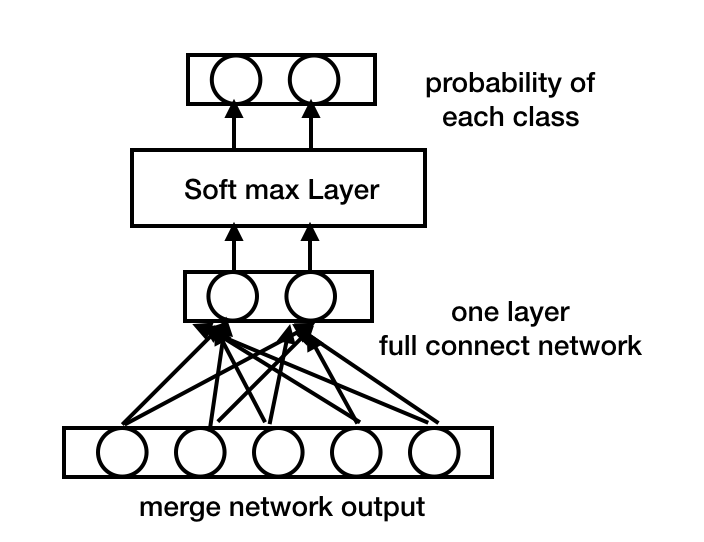
\includegraphics[width=0.5\linewidth]{erfenlei.png}
  \caption{后续接入情感分类网络}
\end{figure}

再如后续网络接入1toM网络,就可以实现一个机器翻译的网络,如下图所示.
把融合网络的输出向量$o$,接到到LSTM中,这样每个隐层的输出$y_{i}$,
就构成了一个序列的向量,进而把每个$y_{i}$映射成字符$w_{k}$,
这样取得了一连串的字符输出,可以作为一个简化的机器翻译网络.

\begin{figure}[h!]
  \centering
  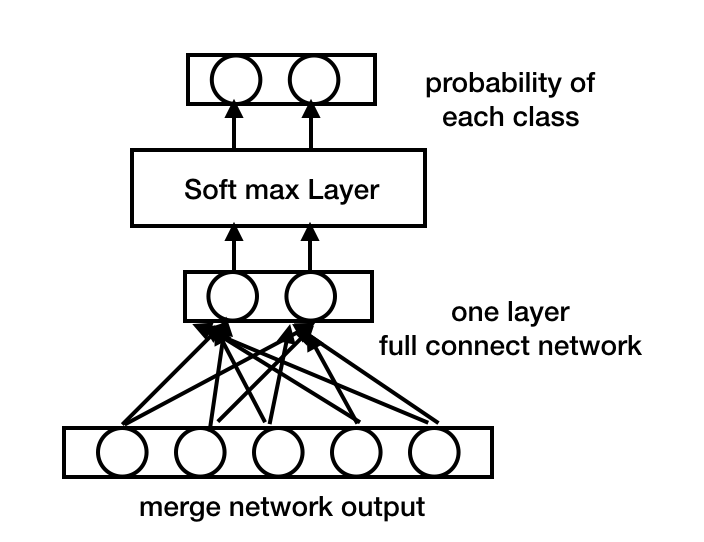
\includegraphics[width=0.5\linewidth]{erfenlei.png}
  \caption{后续接入LSTM网络}
\end{figure}

所以将融合模型的输出$o$,结合先2.2.1小节提到的1 to 1 、1 to N模型,
就可以实现众多的文本理解任务. 

\section{句法结构Attention机制}
句法结构的Attention机制是为了计算出哪个子结构对文本的理解更重要.
所以通过引入Attention机制,可以让网络学习出文本中对整个文本内容相对核心的子结构.
如上一节所说,主要是讨论如何构建打分函数,
得到了当前子结构$m_{i}$,$m_{i} \in \mathbb{R}^{H_{sub}}$与源文本$u$,$u \in \mathbb{R}^{H_{main}}$相关度的评分,
然后采用softmax公式将相关度转换成概率,由此完成了整个Attention机制.
常见的Attention模型包括:dot Attention、bi-liner Attention和concatention-based Attention.

(1)dot Attention

这种Attention机制最为简单,首先需要
构造一个维度平衡矩阵$W$,$W \in \mathbb{R}^{H_{main} \times H_{sub}}$,
所以打分函数可以表示为:

\begin{equation}
  score_{m_{i}} = u^{T}Wm_{i}
\end{equation}

一般采用dot Attention的场合,特别的会$H_{main} = H_{sub}$,这样就只需要点乘即可.

\begin{equation}
  score_{m_{i}} = u^{T}m_{i}
\end{equation}

(2)bi-liner Attention

这个Attention是在dot Attention的基础上构造一个矩阵$W$,$W \in \mathbb{R}^{d \times d}$连续乘其本身和它的转置.
同样一般会有$H_{main} = H_{sub} = d $.

\begin{equation}
  score_{m_{i}} = u^{T}WW^{T}m_{i}
\end{equation}


(3)concatention-based Attention

这个Attention相对比较复杂.
需要构造两个个维度平衡矩阵$W_{1}$,$W_{2}$,
其中$W_{1} \in \mathbb{R}^{d \times H_{sub}}$,
$W_{2} \in \mathbb{R}^{d \times H_{main}}$,
一个偏置向量$b$,$b \in \mathbb{R}^{d}$,
最后还需要一个维度平衡向量$v$,$v \in \mathbb{R}^{d}$.
整个打分函数可以表示如下:

\begin{equation}
  score_{m_{i}} = v^{T}activation(W_{1}m_{i}+W_{2}u+b)
\end{equation}

这里的激活函数一般选择ReLU,tanh即可.



\section{模型融合方式}
这里的融合就是将主文本LSTM的输出的向量$u$,$u \in \mathbb{R}^{H_{main}}$
与表现文本的句法结构的向量$h$,$u \in \mathbb{R}^{H_{sub}}$融合,
为了简化操作,这里假设$u$与$h$的维度是相同的,即$H_{main} = H_{sub}$.
事实上如果不相同,也只需要对于任意一个向量左乘一个平衡矩阵即可.
常见的融合方式,主要有相加融合和连接融合.

(1)相加融合

相加融合,顾名思义就是将$u$和$h$相加.

\begin{equation}
  o = u + h
\end{equation}

当然,这里也可以是有权重的相加,权重表现重要程度的不同.设权重系数为$\alpha$.
这里的$\alpha \in (0,1)$.

\begin{equation}
  o = \alpha u + (1-\alpha)h
\end{equation}

经验上,$\alpha$和模型效果的关系总体上服从先增加后减少的趋势,
所以通过实验可以搜索到对于某个特定任务上最佳的值.

(2)连接融合
连接融合,又可称为串联融合,是把两个向量直接在空间上串行拼接成一个新的向量,
这样新的向量的维度就是原先的两倍,所以需要在通过压缩矩阵$W$,$W \in \mathbb{R}^{d \times 2d}$,
把新的向量压缩成原来的维度.值得注意的是,这里的参数的$W$,也是一个需要学习的变量,不是模型设计初期就固定的.
融合方式具体如下图所示:
\begin{figure}[h!]
  \centering
  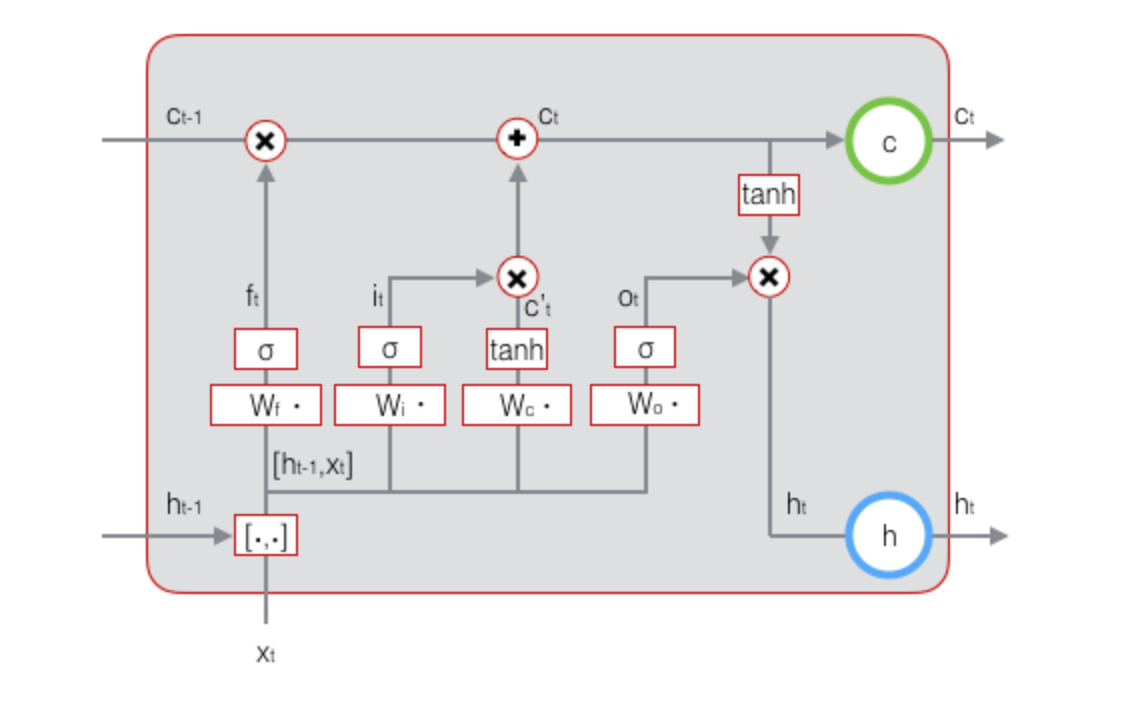
\includegraphics[width=0.4\linewidth]{LSTM.png}
  \caption{连接融合}
\end{figure}

对应到本模型上,连接融合就是是将两个向量串联,即$[u,h]$,最后再左乘$W$,
将其映射为原先的维度,公式如下:

\begin{equation}
  o = W[u,h]
\end{equation}

相加融合和连接融合是目前广泛应用的两种融合方式,在实践上
简单易行而且也能获得比较好的融合效果.
通过融合就能获得文本语义和文本结构的融合表示$o$,进而送入后续的网络中以完成不同的应用.


\chapter{聚类算法分析}
大数据不仅引起学术界和产业界的普遍重视,更上升为世界各国的国家战略.
然而,要充分发挥大数据的作用,必须具备强大的数据分析能力.
本章就无监督学习中的$K-means$算法进行研究,并分析算法的优缺点.
并将本章研究的算法运用到下一章节对具体数据进行聚类分析.

\section{聚类算法}
\subsection{简介}
什么是聚类呢?《周易·系辞上》说:“方以类聚,物以群分,吉凶生矣.”
聚类是把一个数据对象的集合划分成簇(子集),使簇内对象批次相似,
簇间对象不相似的过程,是大数据分析的基本工具.

机器学习包括监督学习和无监督学习.
监督学习的主要任务是分类,即用大量已标记数据完成对新数据的区别;
无监督学习的主要任务是聚类,即在没有任何人工干预情况下对数据进行区分.
无监督学习是大数据分析最基本的工具,
我们必须清楚的看到无监督学习难度远大于监督学习.


\subsection{聚类算法分类}
和分类(监督学习的主要任务)不同,
聚类是在无标记样本的条件下将数据分组,
从而发现数据的天然结构.聚类在数据分析中扮演重要的校色,
它通常被用于以下三个方面:

(1)	发现数据的潜在结构:深入洞察数据、产生假设、检测异常、确定主要特征.

(2)	对数据进行自然分组:确定不同组织之间的相似程度(系统关系).

(3)	对数据进行压缩:将聚类原型作为组织和概括数据的方法.

这几个方面的功能是聚类既可以作为预处理程序,又可以作为独立的数据分析工具.

通过查阅文件和上网查找资料,总结了聚类的发展阶段如下图所示:

\begin{figure}[h!]
  \centering
    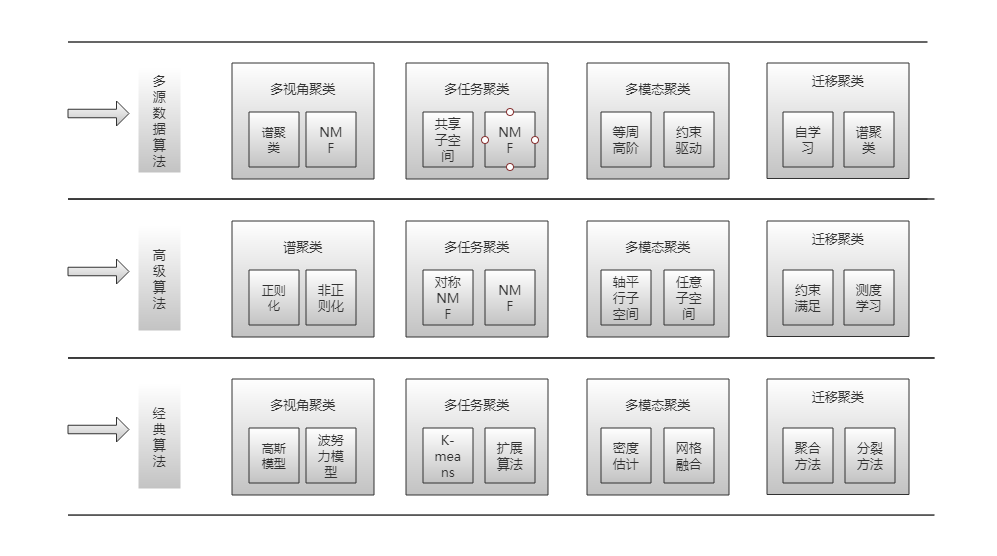
\includegraphics[width=1.0\linewidth]{Wjuleifazhan.png}
  \caption{聚类发展}
\end{figure}


\section{$K-means$算法}
\subsection{算法简介}
$K-means$算法【1】【2】是由Steinhaus与1955年、
Lloyd于1957年、Ball和Hall于1965年、
Mcqueen于1967年分别在各自的不同的科学研究领域独立提出来的.
自被提出来以来,这一算法在许多学科领域得到了大量的研究和应用,
具体的例如数据压缩、数据分类、密度估计等诸多方面.
由于其算法思想简洁易懂,
而且对于许多聚类问题都可花费较小的计算代价而得到不错的聚类结果,
$K-means$算法成为各种聚类算法中较为常用的算法之一,
至今仍然被广泛的使用,被学者们选为数据挖掘领域的十大算法之一【3】.

\subsection{算法思想}
$K-means$算法继承了基于划分的聚类方法的基本思想.
基于划分的算法按某种目标将数据集划分成若干个组,
划分的结果就是使目标函数值最大化(或者最小化).
这样的优化目标通常是NP难的,因此采用某种贪心策略迭代求解.
具体的做法就是每个簇指定一个或者若干个代表点,
根据目标函数用这些代表点对这个数据集进行划分,
在划分结果中重新选择代表点,重复上述过程知道收敛.
贪心算法通常获得目标函数的局部最优解.
基于划分的算法基本上都以点对时间的聚类为标准,
而距离和簇代表点的选择至关重要.

$K-means$算法在如何产生一个划分方面,
$K-means$算法设定了每个划分的中心点,
从而形成以中心为分类依据的球星簇;
在验证所产生的划分是否合理方面,
$K-means$算法以划分的类内紧致性作为标准,
具体来说,是以点与点之间的距离之和作为度量准则.
这种划分标准以及度量标准保证了算法可以很快达到收敛,
这就是$K-means$算法相比于其他算法的一个重大优势.

\subsection{目标函数}
在K-menas算法中,
涉及计算每个对象与各个簇中心点之间的距离,
这个距离的度量也是用户自行设定的.
通常有闵可夫斯基、曼哈顿距离(L1范式)和欧几里得距离(L2)范式等.
针对不同的数据类型可以选取不同的距离度量标准.
在一般情况下,欧几里得是一个很好的度量数据间相似的标准,
也是大部分$K-means$算法中选定的距离度量标准.

聚类算法的目标通常用一个目标函数来表示.
采用欧几里得距离度量相似性的$K-means$算法,
使用误差的平方和(sum of squared errors,SSE)作为度量聚类质量的目标函数.
给定一个包含 $n$ 个数据对象的数据集合$D =\{ x_1, x_2, \cdots, x_n \}$,
定义经由$K-means$算法进行聚类分析后的产生的类别集合为$C=\{ C_1, C_2, \cdots, C_k \}$.
算法目标定义如下:
\begin{equation}
  \centering
  SSE(C) = \sum_{ k=1}^{n} \sum_{x_i \in C_k} {\parallel x_i - c_k \parallel}^2 \qquad 
\end{equation}
式中,$c_k$是簇$C_k$的中心点,计算方法如下所示:

\begin{equation}
  \centering
  c_k = \frac {{\sum_{x_i \in C_k}^{n}} x_i} {\mid C_k \mid} \qquad
\end{equation}

$K-means$算法的目标就是能找到能最小化$SSE$的聚类结果,
这个最优化问题是一个NP难问题【4】,
难以找到一个多项式算法对其求解.
不过可以将此问题进行转化,
通过不断迭代更新簇的构成和簇的中心点来进行最优化的求解,
Lloyd算法就是此类算法.算法的迭代过程主要是:
第一步分配过程,在分配过程中,
每个数据样本都要被分配到离它距离最近的类中心所属的类中;
第二部更新过程,在更新过程中,类的中心点需要被重新计算
,采用分配到这一类别的所有样本数据对类中心点进行更新.
Lloyd算法页被称为精确的$K-means$算法.

那么在簇中心的更新过程中,为什么要选取均值作为计算标准呢?
为什么不是选择中位数等其他标准呢?
下面就从数学角度对这一问题做出详细的说明.
当邻近函数是欧几里得距离且目标是最小化SSE时,
选取均值点作为K-menas算法的簇中心点是可以从数学上推导出来的.
定义$C_k$为第$k$个簇,$x_i$是从属于$C_k$的数据点,
$c_k$是$C_k$中所有数据点的均值点.简化式(4-1),对于一维数组,
式可以写成

\begin{equation}
  \centering
  SSE(C) = \sum_{k=1}^{k}\sum_{x \in C_k}\left(c_k-x_i\right)^2
\end{equation}

为最小化$SSE$,对式(4-3)求导,令导数等于0,并求解$c_k$.其过程如下所示:

\begin{equation}
  \centering
  \frac{\partial SSE}{\partial c_j} = 
  \frac{\partial \sum_{k=1}^{k}\sum_{x \in C_k}\left(c_k-x_i\right)^2}
  {\partial c_j} = \sum_{k=1}^{k}\sum_{x \in C_k} 
  \frac{\partial \left(c_k-x_i\right)^2}{\partial c_j} = 
  \sum_{x_i \in C_j} 2 \cdot \left(c_j - x_i\right) = 0
\end{equation}

\begin{equation}
  \centering
  \sum_{x_i \in C_j} 2 \cdot  \left( c_j - x_i \right) = 0 
  \Rightarrow 
  \vert C_j \vert \cdot c_j = \sum_{x_i \in C_j} x_i 
  \Rightarrow 
  c_j = \frac {\sum_{x_i \in C_j} x_i }{\vert C_j \vert}
\end{equation}

经过以上的推导,最终得出的结果就是当导数为0时,
每个类中心的计算公式正好为计算该类中包含的所有数据点的均值公式,
因此,可以得出这样的结论:簇的最小化SSE的最佳中心点就是簇中各点的均值.


\section{算法流程}
\subsection{算法流程图}
$K-means$算法采用了贪心算法,迭代的方式对聚类结果进行更新,
最终获得最小化的SSE.从某种某种角度上来说,$K-means$算法时EM算法的一种特例,
两者的思想都是先固定一个变量在对另一个变量进行更新,如此反复直到收敛为止.
算法流程如如下所示:

\begin{figure}[h!]
  \centering
    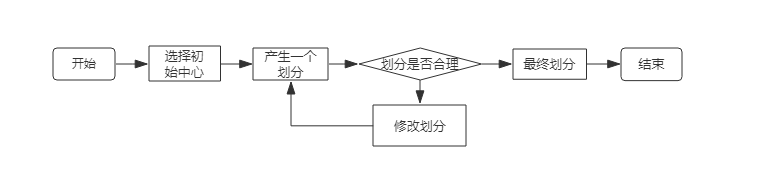
\includegraphics[width=1.0\linewidth]{Wsuanfaliuchengtu.png}
  \caption{算法流程图}
\end{figure}





\subsection{算法步骤}

$K-means$算法采用了贪心算法的思想,以迭代的方式对聚类结果进行更新,
最终获得最小的$SSE$.从某种角度来说,$K-means$算法是$EM$算法的一种特例,
两者的思想都是先固定一个变量然后在对另一个变量进行更新,如此反复直到收敛.
算法4.3给出了$K-means$算法的具体步骤: 

  

\begin{algorithm}[htb]   
  \caption{ $K-means$}   
  \label{alg:Framwork}   
  \begin{algorithmic}[1] %这个1 表示每一行都显示数字  
  \REQUIRE ~~\\ %算法的输入参数:Input  
  All the set of point, $A$;\\  
  The number of clusters, $k$.\\   
  \ENSURE ~~\\ %算法的输出:Output  
  $k$ cluster center points.\\
  \STATE Randomly select k initial center points;    
  \STATE  \textbf{repeat} 
  \STATE \ \ \ \ Calculate the distance between each point and its own center point; \\
  \STATE \ \ \ \ Assign the points to other clusters with the closest distance to your center;
  \STATE \ \ \ \ By formula (4-5) obtained $c_k$, update the cluster center point;
  \STATE  \textbf{until}  The center point does not change;
  \RETURN $k$ coordinate. %算法的返回值  
  \end{algorithmic}  
  \end{algorithm}  


\section{算法实现与分析}
\subsection{算法实现}
在$K-means$算法的实际执行过程中,
可能会出现已经进行了多次迭代而构成的簇还在发生变化的情况.
由于大部分的收敛都发生在早期阶段,在问题要求不是特别严格的情况下,
通常采用一种较弱的条件来替换算法的标准收敛条件,
例如“直到仅有1\%的点发生改变”,
这样弱化的收敛条件可以避免算法迭代次数过多的问题的发生,
在算法的精确性和时间效率上做出了一个平衡.算法执行构成如下图所示。

\begin{figure}[h!]
  \centering
  \begin{subfigure}[b]{0.4\linewidth}
    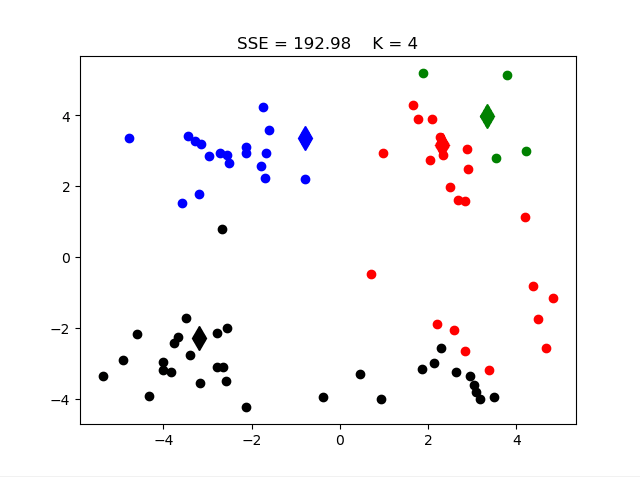
\includegraphics[width=\linewidth]{W4-1.png}
    \caption{第一次迭代}
  \end{subfigure}
  \begin{subfigure}[b]{0.4\linewidth}
    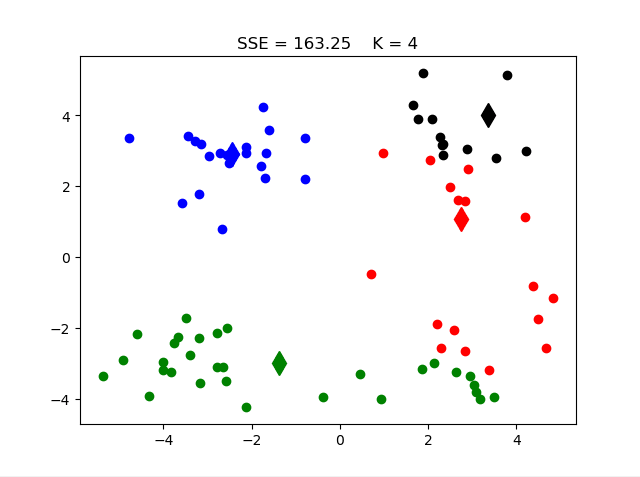
\includegraphics[width=\linewidth]{W4-2.png}
    \caption{第二次迭代}
  \end{subfigure}
  \begin{subfigure}[b]{0.4\linewidth}
    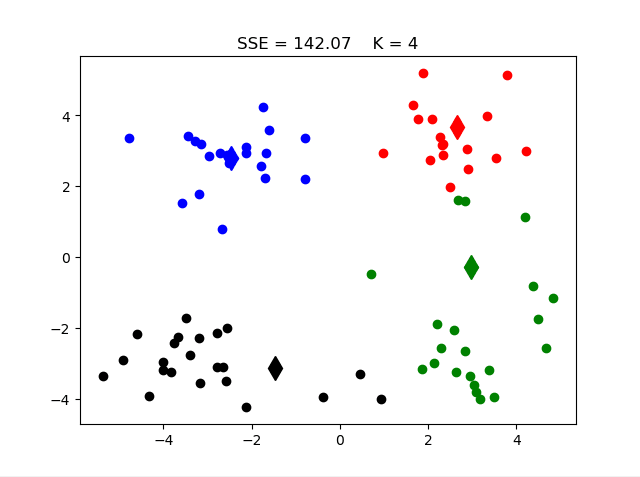
\includegraphics[width=\linewidth]{W4-3.png}
    \caption{第三次迭代}
  \end{subfigure}
  \begin{subfigure}[b]{0.4\linewidth}
    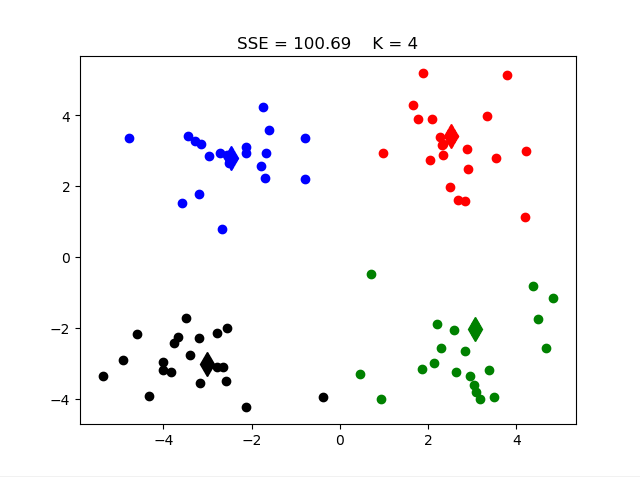
\includegraphics[width=\linewidth]{W4-4.png}
    \caption{第四次迭代}
  \end{subfigure}
  \begin{subfigure}[b]{0.4\linewidth}
    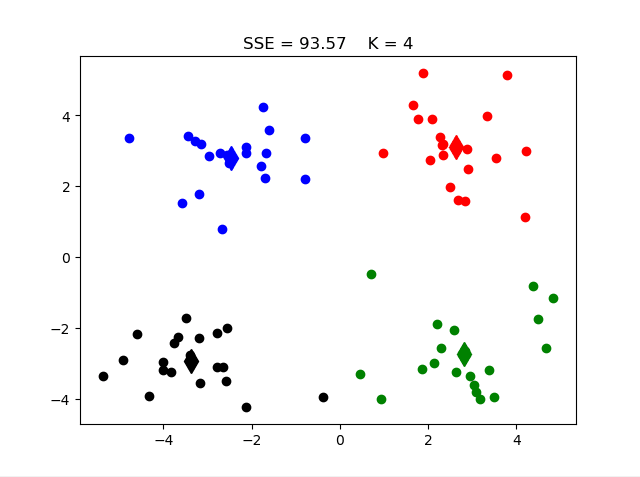
\includegraphics[width=\linewidth]{W4-5.png}
    \caption{第五次迭代}
  \end{subfigure}
  \begin{subfigure}[b]{0.4\linewidth}
    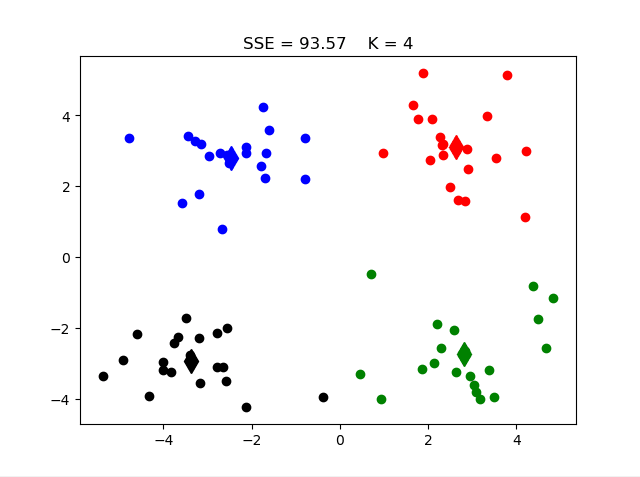
\includegraphics[width=\linewidth]{W4-6.png}
    \caption{第六次迭代}
  \end{subfigure}
  \caption{$K-means$算法执行过程}
\end{figure}

下面举例说明$K-means$算法是如何工作的.
如图4-3所示,数据集中一共包含四个类型的数据点,设定初始聚类个数为4.
首先,随机选取4个初始的中心点,即图中的钻石点.
接下来对于每个数据点,
计算它们与4个中心点的距离并选择最小的那个中心点,加入其表示的簇.
在是有数据点都分配完成后,计算每个簇中所有数据点的均值,
以此作为新的中心点,之后再次进行计算数据点与中心点之间的距离
来进行数据的重新分配,就形成了一次迭代后的数据分配.
重复进行分配和中心点更新这两个步骤,直至簇不在发生变化,
算法终止.如图4-3所示,(a)到(e)图中的中心点不点变化,
就是对中心点的不断更新,其中的有的数据点不断变化的颜色就是在进行重新分配,
直到(e)图,(e)图和(f)图是一样的,说明簇不在发生变化,算法终止.



\subsection{性能分析}
下面对$K-means$算法的性能进行分析,主要是对算法的时间复杂度和空间复杂度进行分析。
\begin{figure}[h!]
  \centering
  \begin{subfigure}[b]{0.8\linewidth}
    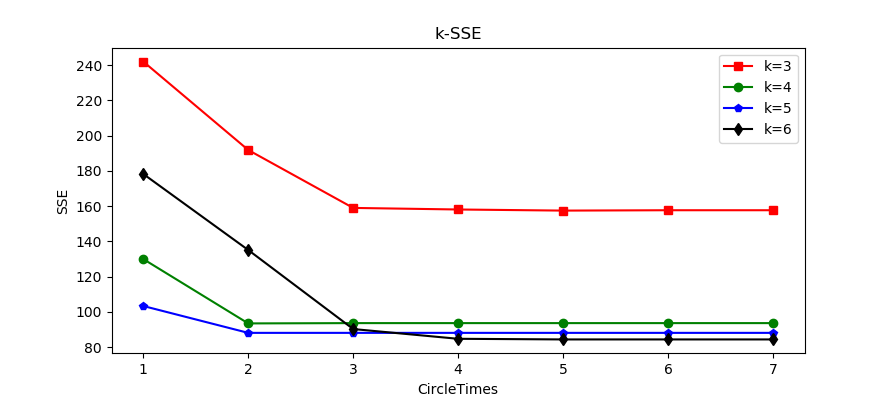
\includegraphics[width=\linewidth]{Wct-SSE-first.png}
    \caption{实验1 k-SSE迭代图}
  \end{subfigure}
  \begin{subfigure}[b]{0.8\linewidth}
    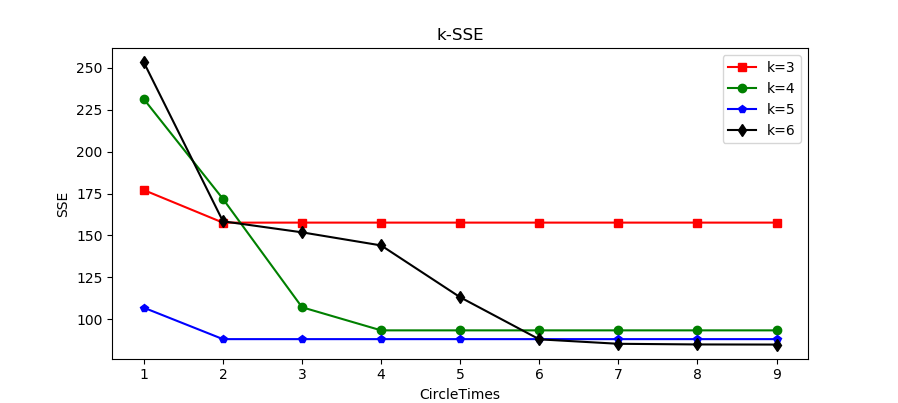
\includegraphics[width=\linewidth]{Wct-SSE-second.png}
    \caption{实验2 k-SSE迭代图}
  \end{subfigure}
  \caption{性能分析}
\end{figure}

在时间方面,$K-means$算法的时间需求基本上与数据点的个数成线性相关。
具体来说,其时间复杂度为$O(i*k*n*m)$,这里的$k$是簇的个数,
$i$是迭代次数(CircleTimes),n是数据集中包含数据点的个数,
m是每个数据的属性数。由于收敛大多发生在早期阶段,$i$的值通常比较小,
如上图所示,$i$为4就收敛了。这样,只要簇的个数$k$远小于$n$,
算法的计算时间就与$n$成线性相关。

在空间方面,$K-means$算法需要存放的类容只有数据点和每个簇的中心点数据。
具体来说,其空间复杂度为$O((k+n)*m)$,
这几个量的定义与计算时间复杂度时的定义一样。
一般可以认为,$i$,$k$和$m$都是常量。
这样的话,算法的时间复杂度和空间复杂度都可以简化为$O(n)$,即线性的。

由此可以看出,$K-means$是一种计算简单而又行至有效的聚类算法。

除了简单且有效以外,$K-means$算法还具有以下优点:

(1)算法使用于各种数据;

(2)当潜在的簇是凸的,
簇与簇之间大小相近且差异明显时,算法可以展现很好的聚类效果;

(3)对于大规模数据集合,该算法非常高效且伸缩性较好

但是,$K-means$算法还存在一些不足之处:

(1)首先,由于在中心点的更新步骤中,算法所使用的是簇内所包含的所有数据点的平均值。
如果在某一问题上无法定义簇内数据点的平均值,那么该算法无法发挥效果。
也就是说,该算法在处理具有分类属性的数据是就无从下手。

(2)在算法的初始化过程中,簇个数$k$的值和初始中心点的选取都对算法结果有着巨大的影响,
不合适的初始化值设定很容易造成算法最终收敛到局部最优值,这使得算法对先于知识具有较强的依赖性。

(3)算法对噪声点和离群点十分敏感,少量的异常数据就会对簇类平均值的计算造成巨大的干扰,
这种干扰很可能会造成簇划分不合理。

针对以上不足,我们可以从算法层面上对标准的$K-means$算法做出修改,
或是在初始化阶段完善对初始值的设定。
在接下来的的一节中,就改进初始化策略做出说明,提高了原有算法的性能,使算法具有更强的生命力。


\subsection{初始的选择}
对于$K-means$算法,有几个十分重要的因素影响着算法的聚类效果,
其中包括簇数目的选定、初始中心点的选取、距离度量的选择以及收敛条件的设定。
距离度量和收敛条件在本节之前已经说明过,余下两项就是在算法的最初阶段决定的,
这两个部分的初始化会直接影响最终能否得到合适的簇。


\begin{figure}[h!]
  \centering
  \begin{subfigure}[b]{0.4\linewidth}
    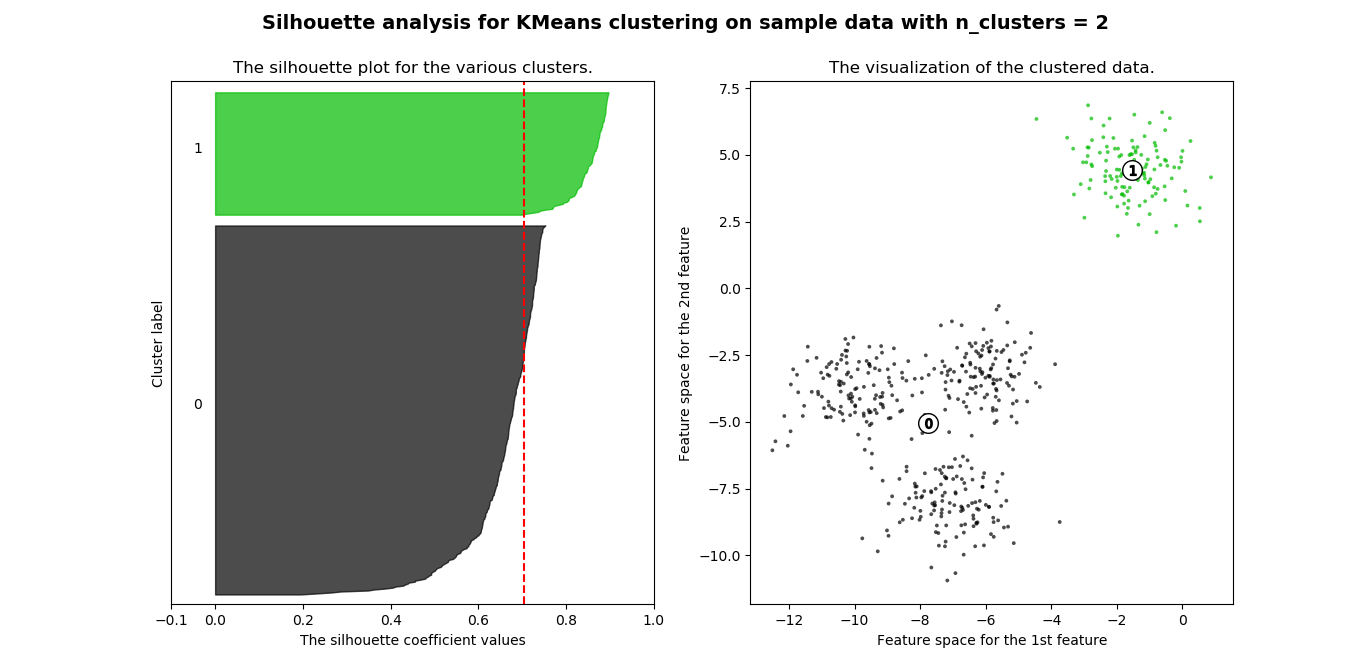
\includegraphics[width=\linewidth]{Wksh-2.png}
    \caption{k=2}
  \end{subfigure}
  \begin{subfigure}[b]{0.4\linewidth}
    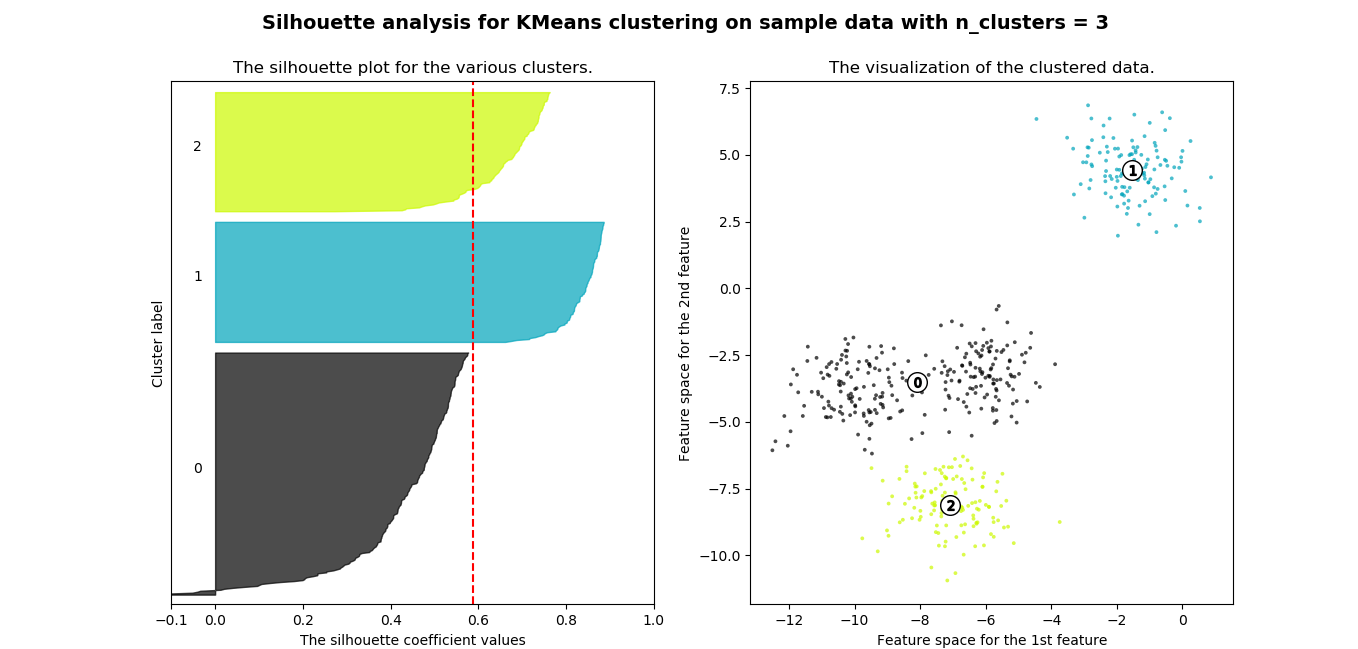
\includegraphics[width=\linewidth]{Wksh-3.png}
    \caption{k=3}
  \end{subfigure}
  \begin{subfigure}[b]{0.4\linewidth}
    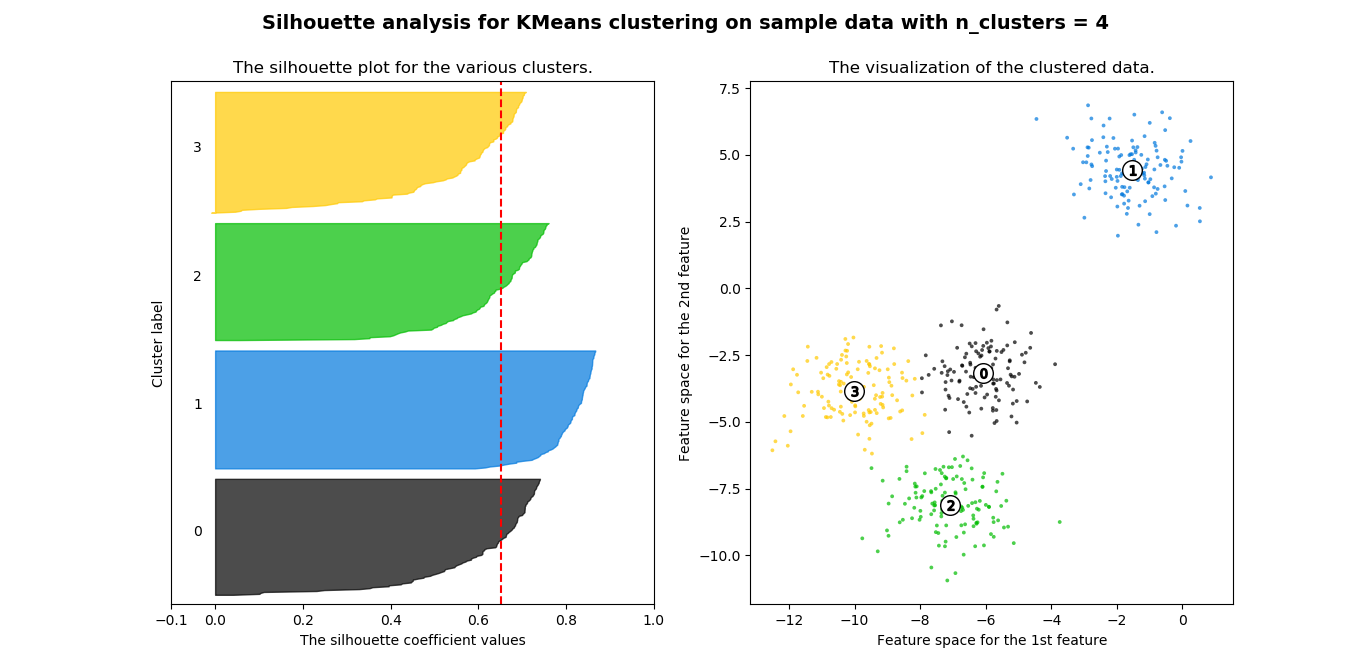
\includegraphics[width=\linewidth]{Wksh-4.png}
    \caption{k=4}
  \end{subfigure}
  \begin{subfigure}[b]{0.4\linewidth}
    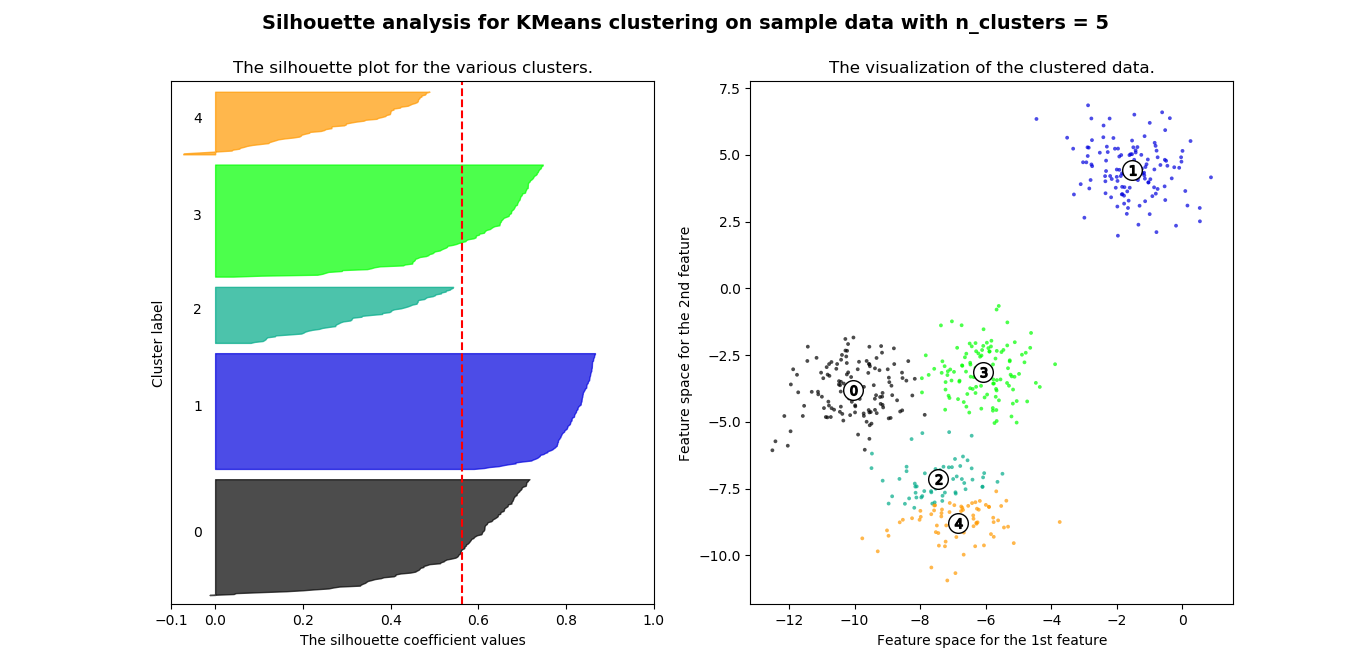
\includegraphics[width=\linewidth]{Wksh-5.png}
    \caption{k=5}
  \end{subfigure}
  \begin{subfigure}[b]{1.0\linewidth}
    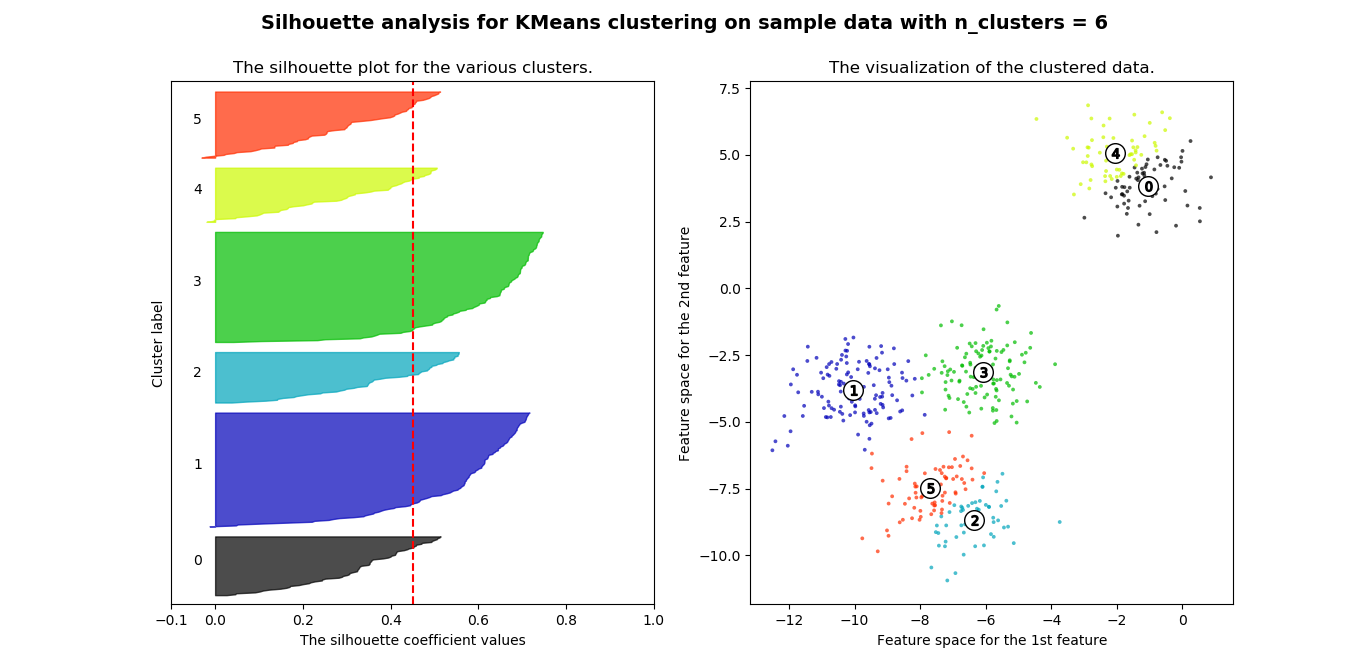
\includegraphics[width=\linewidth]{Wksh-6.png}
    \caption{k=6}
  \end{subfigure}
  \caption{数据可视化}
\end{figure}

$K-means$聚类算法最被人诟病的是类别个数k的选择,
这个设定往往会对结果造成很大的影响,为此提出了一种可行的方法。
该方法是设定一个最大阈值,
令k从小到大逐渐增加,观察SSE的变化从而选取合适的k。
因为k-均值算法中的目标函数是距离的平方和,随着k的增大,
每个簇的类别相似性也随之增加,由此造成SSE的变化是单调的减小。
如果以算法目标为基准,选取使SSE最小的k,
则当k取最大值,即k为数据集中数据个数的时候对应SSE最小。
但这样做是毫无意义的,因为每个数据对对象单独成一个簇。
这种变化来确定SSE的方法中,需要绘制k-SSE折线图,如图4.4所示。
观察图像,在最初k很小的时候,k的增大会使SSE的值迅速减小,之后趋于平缓。
因此,选取图像中的拐点附近的值作为k的起始值,就可以得到很好的聚类效果。


\begin{figure}[h!]
  \centering
    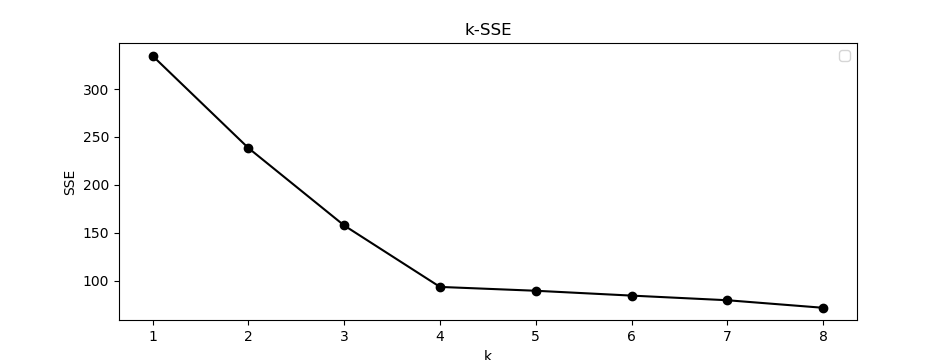
\includegraphics[width=0.8\linewidth]{Wk-SSE.png}
  \caption{k-SSE折线图}
\end{figure}



当然还有其他方法,如Calinski和Harabasz提出的Calinski-Harabasz指标【5】、
Tibshirani等提出的计算差异量统计值方法【6】、
赤池信息准则(akaike information criterion,AIC)【7】、
贝叶斯信息准则(Bayesian information criterion,BIC)【8】、
Newman和Girvan提出一种以结合层次聚类方法的k选取法【9】、
Ball和Hall提出一种迭代自组织的数据分析算法——ISODATA【10】等方法。
本文就不介绍了,有兴趣的话可以查阅相关资料。

上文介绍的是k值的选取,
还有一个重要选择的就是初始点的选择。
最基本的初始点的选取方式就是随机选取k个点作为初始中心点,
这是Macqueen提出的方法【1】。
然而这种方法很容易造成算法最终陷入一个局部最优的解,所得到的聚类分布并不是最优的。
针对这样的问题,
本文采用的一种有效的方法就是选取初始点是先从数据集中随机抽取一些子样本集,
对每一个子样本及都实施随机选取初始中心点的$K-means$算法【12】。
将算法运行后产生的中心点放到一个集合当中,构成一个仅由中心构成的集合,
对这一集合进行聚类分析,将的带的结果作为原数据集的初始中心点。



当然不只这一中有效方法,还有两种方法,一种是将$K-means$算法与聚合层次聚类方法相结合【11】,
另一种是采用最近邻密度的观点。本文对这两种方法也不做详细的介绍。






\rule{\textwidth}{0.5pt}


\chapter{结论与展望}
\section{结论}
文本内容理解作为自然语言处理领域的一项核心技术,其研究在理论和实际应用
上都有重要的意义.
文本内容理解的主要任务是对序列建模,构建模型可以“学习”文本内在的表示特征.
当前基于RNN、LSTM等深度学习模型已经成为了主流方式,但是这种方式忽略了文本自身的语言学知识,
需要非常大的数据集而且缺乏可解释性和鲁棒性.

本文的主要工作是提出了融合依存句法结构的深度神经网络模型,并将模型运用的文本分类的具体应用上,
比传统的神经网络模型取得了更好的效果.

总的来说,通过文本分类的实验,可以看出融合模型具有下面几个优势:

(1) 因为融合模型学习了语言学知识,
所以在小规模数据集上融合模型的实验效果相对于RNN、LSTM模型有明显的提升,测试集上准确率提升3.1\%,
在大数据集上融合模型也具有有优势,测试集准确率最高提升2.5\%.

(2)通过引入Attention机制使得模型可以可视化出在
分类任务上文本中每一个子结构的重要程度,也就进一步可以可视化出
文本中的每一个单词的重要程度.通过可视化文本Attention的热力图,
使得模型具备一定的解释性.

(3)该模型引入依存句法作为语言学知识,
将融合模型的输出结果融合向量表示,可以送入后续任何形式的网络中,
来完成众多不同的文本理解任务.
并且该模型可以无缝替换原先的RNN、LSTM模型,因为融合模型和其输入输出形式完全相同,
所以可以很方便的升级原先的模型,将语言学知识引入原先的模型中.

本文还对模型的Attention方式和融合方式进行了深入的研究,实验表明
采用concatenation-based Attention和加权融合能产生最好的实验结果,
相对LSTM模型提升了2.5\%的准确率.

\section{不足与展望}
因为文本内容理解本身就是一件复杂的研究领域,所以由于条件和时间等方面的原因,
本文的方法还存在需要改进和完善的地方,主要如下:

(1)该模型目前仅仅在在文本分类的任务上进行了实验,还未在更多的文本内容理解任务上实验,
所以可能在某些其他任务上实验效果会不如人意.
尤其对于中文依存句法的解析效果目前还不如英语,所以本模型在处理中文语境下可能会较差,
当然这需要进一步实验来改进调整模型.

(2)该模型由两个独立的LSTM模型和依存句法解析工具构成,所以模型复杂度较高,
在在线处理文本上实时性相对于传统RNN、LSTM模型较差.
主要性能瓶颈在句法解析上,所以未来可能考虑将句法解析融入网络中,
或者引入性能更高的句法解析工具.


% 参考文献.应放在\backmatter之前.
% 推荐使用BibTeX,若不使用BibTeX时注释掉下面一句.
\nocite{*}
\bibliography{bachelor}
% 不使用 BibTeX
%\begin{thebibliography}{2}
%
%\bibitem{deng:01a}
%{邓建松,彭冉冉,陈长松}.
%\newblock {\em \LaTeXe{}科技排版指南}.
%\newblock 科学出版社,书号:7-03-009239-2/TP.1516, 北京, 2001.
%
%\bibitem{wang:00a}
%王磊.
%\newblock {\em \LaTeXe{}插图指南}.
%\newblock 2000.
%\end{thebibliography}

%%%%%%%%%%%%%%%%%%%%%%%%%%%%%%%%%%%%%%%%%%%%%%%%%%%%%%%%%%%%%%%%%%%%%%%%%%%%%%%
% 致谢,应放在《结论》之后
\begin{acknowledgement}
感谢我的毕设导师王澜老师,感谢他在毕设的各个环节对我的提醒、检查和督促.

感谢我的研究生导师黄河燕教授,她让我在本科的最后阶段
接触到了自然语言处理这个领域,并给我提供了开放自由的科研环境,以及对我毕设全程的关心和指导.

还要特别感谢魏骁驰博士,他学识渊博,毕设的从始至终一直一步步指导我完成,
耐心解答了我所有提出的问题.帮助我明晰了每一步需要做什么,具体怎么做,做好了如何完善.
将原本很难的课题,分解成一个个小问题,指导我去解决.
并且他在工作中认真负责,在生活中积极开朗的性格也深深的感染了我.

感谢所有任课老师孜孜不倦地教导,让我在大学四年学到了方方面面的知识.
感谢我的班主任冯伟老师,是他引导我走上科创的道路,并认识了很多优秀的同学.

感谢我的家人,感谢他们对我的无私奉献,是我一直以来的坚强后盾,
帮助我一起面对困难,战胜困难.

最后,真挚的感谢所有给我提供帮助和鼓励的人.
\end{acknowledgement}

\backmatter




%%%%%%%%%%%%%%%%%%%%%%%%%%%%%%%%%%%%%%%%%%%%%%%%%%%%%%%%%%%%%%%%%%%%%%%%%%%%%%%
\end{document}
